%% OXFORD THESIS TEMPLATE

% Use this template to produce a standard thesis that meets the Oxford University requirements for DPhil submission
%
% Originally by Keith A. Gillow (gillow@maths.ox.ac.uk), 1997
% Modified by Sam Evans (sam@samuelevansresearch.org), 2007
% Modified by John McManigle (john@oxfordechoes.com), 2015
%
% This version Copyright (c) 2015-2017 John McManigle
%
% Broad permissions are granted to use, modify, and distribute this software
% as specified in the MIT License included in this distribution's LICENSE file.
%

% I've (John) tried to comment this file extensively, so read through it to see how to use the various options.  Remember
% that in LaTeX, any line starting with a % is NOT executed.  Several places below, you have a choice of which line to use
% out of multiple options (eg draft vs final, for PDF vs for binding, etc.)  When you pick one, add a % to the beginning of
% the lines you don't want.


%%%%% CHOOSE PAGE LAYOUT
% The most common choices should be below.  You can also do other things, like replacing "a4paper" with "letterpaper", etc.

% This one will format for two-sided binding (ie left and right pages have mirror margins; blank pages inserted where needed):
% \documentclass[a4paper,twoside]{ociamthesis}
% This one will format for one-sided binding (ie left margin > right margin; no extra blank pages):
\documentclass[a4paper]{ociamthesis}
% This one will format for PDF output (ie equal margins, no extra blank pages):
%\documentclass[a4paper,nobind]{ociamthesis} 


%%%%%%%%%%%%%%%%%%%%%%%%%%%%%%%%%%%%%%%%%%%%%%%%%%%%%%%%%%%%%%%%
% JR additions to the template

% Newlines lead to a paragraph break, not just an indentation
\usepackage[parfill]{parskip}


% Note: use this link https://greasyfork.org/en/scripts/390507-overleaf-editor-map-j-to-gj-and-k-to-gk
% In combination with tapermonkey to move up and down a single visual line with j and k

% Make sure figures go in the right section
\usepackage[section]{placeins}
%%%%%%%%%%%%%%%%%%%%%%%%%%%%%%%%%%%%%%%%%%%%%%%%%%%%%%%%%%%%%%%

\usepackage[font=footnotesize, singlelinecheck=false]{caption}
\usepackage{graphicx,floatpag,caption}


%%%%% SELECT YOUR DRAFT OPTIONS
% Three options going on here; use in any combination.  But remember to turn the first two off before
% generating a PDF to send to the printer!

% This adds a "DRAFT" footer to every normal page.  (The first page of each chapter is not a "normal" page.)
% \fancyfoot[C]{\emph{DRAFT Printed on \today}}  

% This highlights (in blue) corrections marked with (for words) \mccorrect{blah} or (for whole
% paragraphs) \begin{mccorrection} . . . \end{mccorrection}.  This can be useful for sending a PDF of
% your corrected thesis to your examiners for review.  Turn it off, and the blue disappears.
\correctionstrue


%%%%% BIBLIOGRAPHY SETUP
% Note that your bibliography will require some tweaking depending on your department, preferred format, etc.
% The options included below are just very basic "sciencey" and "humanitiesey" options to get started.
% If you've not used LaTeX before, I recommend reading a little about biblatex/biber and getting started with it.
% If you're already a LaTeX pro and are used to natbib or something, modify as necessary.
% Either way, you'll have to choose and configure an appropriate bibliography format...

% The science-type option: numerical in-text citation with references in order of appearance.
\usepackage[style=nature, sorting=none, backend=biber, doi=false, isbn=false, url=false, eprint=false, maxbibnames=99]{biblatex}
% \usepackage[maxbibnames=99]{biblatex}
% \newcommand*{\bibtitle{References}
% Makes nature style citations, no packages needed
\let\cite=\supercite


% The humanities-type option: author-year in-text citation with an alphabetical works cited.
%\usepackage[style=authoryear, sorting=nyt, backend=biber, maxcitenames=2, useprefix, doi=false, isbn=false]{biblatex}
% \newcommand*{\bibtitle}{Works Cited}

% This makes the bibliography left-aligned (not 'justified') and slightly smaller font.
\renewcommand*{\bibfont}{\raggedright\small}

% Change this to the name of your .bib file (usually exported from a citation manager like Zotero or EndNote).
\addbibresource{references.bib}

% Uncomment this if you want equation numbers per section (2.3.12), instead of per chapter (2.18):
%\numberwithin{equation}{subsection}

%%%%% THESIS / TITLE PAGE INFORMATION
% Everybody needs to complete the following:
\title{
Optical control of neocortical circuits to probe how connectivity influences behavioural salience
}
\author{James Rowland}
\college{Corpus Christi College}

% Uncomment the following line if your degree also includes exams (eg most masters):
%\renewcommand{\submittedtext}{Submitted in partial completion of the}
% Your full degree name.  (But remember that DPhils aren't "in" anything.  They're just DPhils.)
\degree{Doctor of Philosophy}
% Term and year of submission, or date if your board requires (eg most masters)
\degreedate{Trinity 2021}


%%%%% YOUR OWN PERSONAL MACROS
% This is a good place to dump your own LaTeX macros as they come up.

% To make text superscripts shortcuts
	\renewcommand{\th}{\textsuperscript{th}} % ex: I won 4\th place
	\newcommand{\nd}{\textsuperscript{nd}}
	\renewcommand{\st}{\textsuperscript{st}}
	\newcommand{\rd}{\textsuperscript{rd}}

\AtEveryBibitem{\clearfield{month}}
\AtEveryBibitem{\clearfield{day}}
\AtEveryBibitem{\clearlist{language}}
\AtEveryBibitem{\clearfield{note}}
%%%%% THE ACTUAL DOCUMENT STARTS HERE
\begin{document}



%%%%% CHOOSE YOUR LINE SPACING HERE
% This is the official option.  Use it for your submission copy and library copy:
\setlength{\textbaselineskip}{22pt plus2pt}
% This is closer spacing (about 1.5-spaced) that you might prefer for your personal copies:
%\setlength{\textbaselineskip}{18pt plus2pt minus1pt}

% You can set the spacing here for the roman-numbered pages (acknowledgements, table of contents, etc.)
% Need this for TOC but maybe not for abstract
\setlength{\frontmatterbaselineskip}{17pt plus1pt minus1pt}

% Leave this line alone; it gets things started for the real document.
\setlength{\baselineskip}{\textbaselineskip}


%%%%% CHOOSE YOUR SECTION NUMBERING DEPTH HERE
% You have two choices.  First, how far down are sections numbered?  (Below that, they're named but
% don't get numbers.)  Second, what level of section appears in the table of contents?  These don't have
% to match: you can have numbered sections that don't show up in the ToC, or unnumbered sections that
% do.  Throughout, 0 = chapter; 1 = section; 2 = subsection; 3 = subsubsection, 4 = paragraph...

% The level that gets a number:
\setcounter{secnumdepth}{1}
% The level that shows up in the ToC:
\setcounter{tocdepth}{2}

% Comment to count figures as 'chapter.figurenum' not 1,2,3,4 from the start 
\renewcommand\thefigure{\arabic{figure}}
\counterwithout{figure}{chapter}



%%%%% ABSTRACT SEPARATE
% This is used to create the separate, one-page abstract that you are required to hand into the Exam
% Schools.  You can comment it out to generate a PDF for printing or whatnot.
% \begin{abstractseparate}
% 	The brains of higher organisms are composed of anatomically and functionally distinct regions performing specialised tasks. However, individual regions do not operate in isolation. Hence, the orchestration of complex behaviours requires communication between brain regions and reliable transmission of information between them. We study this process directly by generating neural activity that propagates between brain regions and drives behaviour, allowing us to assess how populations of neurons in sensory cortex act in concert to transmit information. We achieved this by imaging two hierarchically organised and densely interconnected regions, the primary and secondary somatosensory cortex (S1 and S2) in mice while performing two-photon photostimulation of S1 neurons and assigning behavioural salience to the photostimulation. We found that the probability of perception is determined by both the variance of the S1 network and the strength of the photostimulation. Conceptually this means that maximising the signal-to-noise ratio of an incoming stimulus is critical to its continued propagation downstream. Further, we show that propagated, behaviourally salient activity elicits balanced, persistent and generalised activation of the downstream region, consistent with inhibitory stabilised network models with dense recurrent connectivity. Hence, our work adds to existing understanding of cortical function by identifying how population activity is formatted to ensure robust transmission of information, allowing specialised brain regions to communicate and coordinate behaviour. % Create an abstract.tex file in the 'text' folder for your abstract.
% \end{abstractseparate}


% JEM: Pages are roman numbered from here, though page numbers are invisible until ToC.  This is in
% keeping with most typesetting conventions.
% \begin{romanpages}

% Title page is created here
\maketitle

%%%%% DEDICATION -- If you'd like one, un-comment the following.
%\begin{dedication}
%This thesis is dedicated to\\
%someone\\
%for some special reason\\
%\end{dedication}

%%%%% ACKNOWLEDGEMENTS -- Nothing to do here except comment out if you don't want it.
\begin{acknowledgements}
 	Umb thanks for the toungey




\end{acknowledgements}

%%%%% ABSTRACT -- Nothing to do here except comment out if you don't want it.
\begin{abstract}
	The brains of higher organisms are composed of anatomically and functionally distinct regions performing specialised tasks. However, individual regions do not operate in isolation. Hence, the orchestration of complex behaviours requires communication between brain regions and reliable transmission of information between them. We study this process directly by generating neural activity that propagates between brain regions and drives behaviour, allowing us to assess how populations of neurons in sensory cortex act in concert to transmit information. We achieved this by imaging two hierarchically organised and densely interconnected regions, the primary and secondary somatosensory cortex (S1 and S2) in mice while performing two-photon photostimulation of S1 neurons and assigning behavioural salience to the photostimulation. We found that the probability of perception is determined by both the variance of the S1 network and the strength of the photostimulation. Conceptually this means that maximising the signal-to-noise ratio of an incoming stimulus is critical to its continued propagation downstream. Further, we show that propagated, behaviourally salient activity elicits balanced, persistent and generalised activation of the downstream region, consistent with inhibitory stabilised network models with dense recurrent connectivity. Hence, our work adds to existing understanding of cortical function by identifying how population activity is formatted to ensure robust transmission of information, allowing specialised brain regions to communicate and coordinate behaviour.
\end{abstract}

%%%%% MINI TABLES
% This lays the groundwork for per-chapter, mini tables of contents.  Comment the following line
% (and remove \minitoc from the chapter files) if you don't want this.  Un-comment either of the
% next two lines if you want a per-chapter list of figures or tables.
\dominitoc % include a mini table of contents
%\dominilof  % include a mini list of figures
%\dominilot  % include a mini list of tables

% This aligns the bottom of the text of each page.  It generally makes things look better.
\flushbottom

% This is where the whole-document ToC appears:
% \tableofcontents

% \renewcommand{\baselinestretch}{0.75}\normalsize
\tableofcontents
% \renewcommand{\baselinestretch}{1.0}\normalsize



\listoffigures
	\mtcaddchapter
% \mtcaddchapter is needed when adding a non-chapter (but chapter-like) entity to avoid confusing minitoc

% Uncomment to generate a list of tables:
%\listoftables
%	\mtcaddchapter

%%%%% LIST OF ABBREVIATIONS
% This example includes a list of abbreviations.  Look at text/abbreviations.tex to see how that file is
% formatted.  The template can handle any kind of list though, so this might be a good place for a
% glossary, etc.
% % First parameter can be changed eg to "Glossary" or something.
% Second parameter is the max length of bold terms.
\begin{mclistof}{List of Abbreviations}{3.2cm}

\item[1-D, 2-D] One- or two-dimensional, referring in this thesis to spatial dimensions in an image.

\item[Otter] One of the finest of water mammals.

\item[Hedgehog] Quite a nice prickly friend.

\end{mclistof} 


% The Roman pages, like the Roman Empire, must come to its inevitable close.
% \end{romanpages}


%%%%% CHAPTERS
% Add or remove any chapters you'd like here, by file name (excluding '.tex'):
\flushbottom
% Useful how to docs etc
\chapter{\label{ch:1-intro}Introduction} 
\minitoc

Key to the orchestration of behaviour by neural systems is that information, in the form of neural activity, is reliably and accurately transmitted between anatomically distinct brain regions performing specialised tasks. Activity is transformed at each stage of its journey, and circuits often perform multiple tasks in parallel \cite{mante_context-dependent_2013, stringer_spontaneous_2019}, so it is challenging to disentangle which facets of neural activity contribute to a specific behaviour or process. In-depth analysis of cellular resolution recordings of neural activity during sensory stimulation \cite{hubel_receptive_1962, simons_response_1978, carandini_linearity_1997, okun_diverse_2015, stringer_high-dimensional_2019}  and/or well-characterised behaviour \cite{britten_analysis_1992, platt_neural_1999, yang_probabilistic_2007, herzfeld_encoding_2015, lak_dopaminergic_2020} has begun to shed light on how the sensory world, decisions and actions are encoded in individual brain regions. However, how activity is structured in order to facilitate its journey through the brain is less well understood. It is especially critical that close attention is paid to unravelling how activity is propagated through the healthy brain, as dysfunction of this process is thought to play a key role in the aetiology of Alzheimer’s disease \cite{hazra_inhibitory_2013, busche_impairments_2016}, Parkinson’s disease\cite{mcgregor_circuit_2019} and epilepsy \cite{goldberg_mechanisms_2013}.

For researchers studying streams of sensory processing, it is advantageous to circumvent the transformations of neural activity occurring at regions upstream from the brain region under study. This can be achieved by taking experimental control of neural activity and driving spikes directly through stimulation of individual neurons \cite{houweling_behavioural_2008, tanke_single-cell_2018, chettih_single-neuron_2019} or groups of neurons \cite{romo_somatosensory_1998, huber_sparse_2008, histed_cortical_2014, dalgleish_how_2020, gill_precise_2020}. The recent renaissance in optical methods enables this to be achieved with unparalleled precision and flexibility. Specifically, two-photon optogenetics allows researchers to drive a predefined number of spikes in between one and hundreds of neurons with near single-cell precision, with the identities and number of neurons stimulated varied on a trial-by-trial basis. Neural responses can vary trial-by-trial to even identical sensory stimulus presentations \cite{britten_responses_1993, faisal_noise_2008, softky_highly_1993}, rendering the flexibility endowed by two-photon optogenetics critical for tightly controlling the evoked response in the sensory stream and observing its effect on behaviour. Moreover, direct experimental stimulation of neurons is likely a critical tool for understanding activity propagation, as the activity of anatomically connected brain regions is typically highly correlated \cite{honey_predicting_2009, musall_single-trial_2019}, but it is often unclear whether this correlated activity results from propagation between regions or from common input. Direct stimulation circumvents this issue as activity locked temporally to stimulation of a connected region likely arises from propagation. Thus, we can understand how connected brain regions coordinate by directly stimulating a given brain region, and recording a connected region, during behaviour that is causally underpinned by propagating activity.

To approach this problem, my colleagues and I imaged two hierarchically organised, densely interconnected and functionally well-characterised \cite{pons_physiological_1987, kamatani_experience-dependent_2007, aronoff_long-range_2010, chen_behaviour-dependent_2013, yamashita_membrane_2013, chen_long-range_2016, kwon_sensory_2016, yamashita_target-specific_2016} regions, the primary and secondary somatosensory cortex (S1 and S2) while performing two-photon optogenetic photostimulation of S1 neurons. We assigned behavioural salience to photostimulation by training mice through operant conditioning to report detection of the stimulation. Photostimulation was targeted to varying groups of 5-150 neurons in S1, allowing us to parametrically adjust the effect of photostimulation, monitor its effect on behaviour and record trials spanning the perceptual threshold of the animal. By simultaneously recording neural activity occurring before and after photostimulation in both brain regions, we were able to assess how behaviourally salient stimulation is propagated through anatomically distinct brain regions.

We demonstrate that behaviourally salient photostimulation of S1 (hit trials) elicits robust activation of S2, which represents stimulus information for several seconds after stimulation. Further, we find that ongoing activity in S1 and S2, immediately preceding stimulation, influences the detectability of the upcoming stimulus. Specifically, the photostimulus detectability and propensity to propagate is greatest when both the population variance pre-stimulus in S1 is minimised and the number of cells stimulated is maximised. This is consistent with a signal-to-noise framework in which the signal is the number of photostimulated cells and the noise is the variance of the ongoing activity in S1. Thus we demonstrate that the signal-to-noise ratio of an input to a neural circuit is critical both for the behavioural salience of the input and the likelihood that the input is reliably propagated beyond the brain region in which it arises.

In this project I developed, alongside my colleagues, a novel preparation which allowed us to simultaneously read and write propagating neural activity in the mouse. This was achieved by combining single-cell resolution two-photon calcium imaging of neural activity propagating between cortical regions, and two-photon optogenetic stimulation of small groups of neurons which causally drove behaviour. To run these experiments, I built both hardware and software to run behavioural training and optogenetic stimulation in an automated manner, requiring minimal experimenter intervention during sessions and which automatically progressed mice through stages of training. During the final stages of training, optogenetic stimulation was delivered using holographic two-photon photostimulation, a cutting-edge optical method which has not previously been used in a preparation spanning multiple brain regions. Finally, I performed transformations and in-depth statistical modelling of the resulting data to draw conclusions about cortical function.

In this thesis, I introduce the methods and biological theory that underpin the project, outline how these techniques are employed in our novel preparation, and explain how we performed statistical modelling to draw conclusions from the data. Finally I set these findings in the context of the field and explore how they might act to advance our understanding of the neural code.

\section{Recording neural activity}

Cortical computation is likely underpinned by populations of neurons  rather than individual neurons acting in isolation \cite{averbeck_neural_2006, kohn_correlations_2016, panzeri_cracking_2017}. Hence, to understand neural coding in cortex, it is necessary to record the activity of large groups of neurons simultaneously \textit{in vivo}. These recordings were first carried out through electrical methods in which one or more microelectrodes are inserted into the extracellular space around neurons, allowing the action potential waveform to be recorded from multiple cells \cite{hubel_tungsten_1957, mcnaughton_stereotrode_1983, buzsaki_large-scale_2004}. Recent developments to this technique have resulted in electrodes capable of recording hundreds of neurons simultaneously, through thousands of channels, with exquisite temporal resolution \cite{steinmetz_neuropixels_2021}. However, despite the power of this method, it has a number of drawbacks. It is often not possible to track the genetic identity or spatial relationship of recorded cells, analysis to parcel out recorded activity to individual neurons is complex \cite{harris_improving_2016}, and stimulation of neurons during electrical recordings is limited to single-cell stimulation \cite{margrie_vivo_2002, houweling_nanostimulation_2010} or simultaneous activation of groups of spatially co-localised neurons \cite{penfield_w_somatic_1937, asanuma_functional_1967, salzman_cortical_1990, romo_somatosensory_1998, cardin_driving_2009, kim_integration_2017}.

More recently, fluorescence microscopy has been applied to functional imaging \textit{in vivo} to circumvent these issues and record large populations of neurons with single cell resolution. Normally, neural activity is recorded optically using calcium imaging \cite{grienberger_imaging_2012}, in which neurons are genetically engineered to express fluorescent molecules which undergo a conformational change when bound to calcium. As a result, the fluorescence intensity of neurons expressing these molecules increases following calcium influx driven by an action potential \cite{berridge_neuronal_1998} and spikes can be recorded optically. Currently, the most popular way to perform calcium imaging \textit{in vivo} is through genetically encoded calcium indicators \cite{looger_genetically_2012} such as GCaMP \cite{chen_ultrasensitive_2013, dana_high-performance_2019}. These can be expressed in neurons long-term through viral injection \cite{packer_simultaneous_2015} or in transgenic animals \cite{huang_relationship_2021} enabling chronic imaging of the same neurons over time \cite{andermann_chronic_2013}. While calcium imaging addresses the drawbacks of electrophysiology by visualising neurons, the time course of the indicator can span hundreds of milliseconds, meaning it has substandard temporal resolution compared to electrophysiology and resolving single-spike events can be challenging \cite{huang_relationship_2021}. Most germane to this thesis however, calcium imaging is the only method of recording neural populations that has thus far been combined with targeted two-photon photostimulation \cite{packer_simultaneous_2015} (see below).

Fluorescence microscopy \cite{lichtman_fluorescence_2005} requires a light-source to excite the fluorophores in the sample. This often takes the form of an LED or laser which bathes the entire sample simultaneously in light, allowing a sensor, such as a camera, to detect emitted photons and create an image of the sample. This is known as ‘widefield’ or ‘one-photon’ excitation. However, biological tissue is highly scattering, meaning a photon emitted from a given location on the sample may not arrive at the exact corresponding location on the sensor. Additionally illumination causes the specimen to fluoresce throughout the z-dimension, resulting in photons emitted beyond the desired focal plane. Taken together, these phenomena degrade the spatial resolution of the image. By contrast, scanning microscopy creates ‘optical sectioning’ by sampling regions of the sample in sequence, meaning detected photons can be assigned to a known location of the specimen \cite{lichtman_fluorescence_2005}. While confocal microscopy \cite{nwaneshiudu_introduction_2012} is the most popular form of scanning microscopy, it is of little use to \textit{in vivo} mammalian neuroscience, as the wavelengths of light used to excite common fluorophores do not penetrate beyond the most superficial layers of the brain \cite{helmchen_deep_2005}. This issue is circumvented by two-photon microscopy which, usually, employs near-infrared wavelength lasers producing photons of roughly half the energy required to excite the fluorophore in the sample. These long-wavelength lasers penetrate deep into tissue with minimal scattering and generate optical sectioning of the specimen through multiphoton absorption. Multiphoton absorption occurs when two photons arrive simultaneously at the fluorophore and excite it by combining their energies, thus creating optical sectioning as the probability of this event occurring is vanishingly small beyond the focal point of the excitation beam. Hence detected photons can be confidently assigned to a small point on the sample which produces a high-resolution image up to several hundred microns deep in a sample of neural tissue \cite{helmchen_deep_2005}.

Thus by combining calcium imaging with two-photon microscopy, the activity of hundreds of neurons can be recorded in awake behaving mice with minimal tissue lesioning \cite{helmchen_vivo_1999, stosiek_vivo_2003, lutcke_steady_2013, driscoll_dynamic_2017, stringer_spontaneous_2019}.

\section{Manipulating neural activity with light}

Experiments which rely purely on recording neural activity during behaviour can be very challenging to design and interpret as it is unclear which of the sprawling array of brain regions, cell types, projection targets and neural features of interest are driving the behaviour. Hence it is beneficial to perform artificial manipulation or deletion of neural activity and observe its effect on behaviour (but see \cite{otchy_acute_2015} for potential pitfalls with this approach). The current leading method in the neuroscientist’s toolkit to perform these experiments is optogenetics, which combines optical and genetic technology to allow experimenters to take direct control of neurons and neural circuits. Briefly and generally, optogenetic experiments are conducted by engineering a light-sensitive protein (opsin) into a neuron, or other cell type. This allows the experimenter to shine light onto the cell and drive a current which can, for example, increase or decrease a neuron's firing rate (for reviews see \cite{miesenbock_optogenetic_2009, deisseroth_optogenetics_2011}). Optogenetics has unparalleled versatility in that experimenters can deliver loss or gain of function restricted to individual brain regions \cite{zhang_optogenetic_2010}, genetic subtypes \cite{cardin_driving_2009, tye_dopamine_2013, zalocusky_nucleus_2016} or projection targets \cite{mattis_frequency-dependent_2014} in a behaving animal \cite{tye_amygdala_2011} with tight temporal control \cite{krook-magnuson_-demand_2013}. 

However, in a similar vein to the issues raised above with fluorescence imaging, using widefield illumination to drive optogenetic stimulation is spatially imprecise and results in coactivation of hundreds to thousands of neurons simultaneously \cite{huber_sparse_2008}. This likely evokes non-physiological patterns of activity, conflicting with the sparse coding regime that has been observed in cortex \cite{olshausen_sparse_2004}. It is also unlikely that all stimulated neurons can be recorded. Additionally, widefield optogenetics can be targeted only to genetic subtypes of neurons and not to functionally-defined subtypes, which may drive a behaviour but be distributed throughout one or more brain regions.  Finally, the same neurons are likely stimulated on each trial, meaning the effect of stimulation is challenging to vary on a trial-by-trial basis.

Recently, researchers expanded the use of two-photon technology beyond recording neurons to controlling them through optogenetics \cite{rickgauer_simultaneous_2014, packer_simultaneous_2015, hernandez_three-dimensional_2016, mardinly_precise_2018, chettih_single-neuron_2019, marshel_cortical_2019, daie_targeted_2021}. This greatly improves the spatial resolution of the stimulation and hence addresses the issues outlined above. The optical sectioning afforded by a two photon laser beam means that stimulation can be restricted to individual neurons. Additionally the targeted neuron(s) can be visually identified by the experimenter, meaning that, when combined with calcium imaging, functional neuronal subtypes can be identified which, for example, exhibit correlated firing with a specific behavioural event. Thus by photostimulting such neurons, their causal role in the behaviour can be assessed \cite{marshel_cortical_2019, daie_targeted_2021, dalgleish_how_2020, russell_influence_2019}.

While standard two-photon beam paths can be used to target single neurons for photostimulation, targeting multiple neurons requires more specialised optics to split the beam. The most widely used way of achieving this is through digital holography, in which a spatial light modulator (SLM) 	is incorporated into the beam path. Through a reflective liquid-crystal layer, this acts as a programmable two-dimensional diffraction grating, allowing arbitrary patterns to be created from the two-photon beam \cite{lutz_holographic_2008}. Thus, the researcher is able to target arbitrary combinations of neurons for optogenetic manipulation, changing the identify, combination or quantity of targets on a trial-by-trial basis. 

Recently, the toolkit of opsins available to researchers has expanded to include proteins particularly suited to \cite{yizhar_neocortical_2011} or specifically designed for \cite{chettih_single-neuron_2019, mardinly_precise_2018, marshel_cortical_2019} two-photon optogenetic experiments. Two specific advances utilised in this thesis are the development of opsins with a red-shifted excitation spectrum, and opsins with somatic-targeting motifs. Red-shifted opsins are useful as they can be used  simultaneously with fluorescence imaging of proteins excited by blue light (such as GCaMP). Somatic-targeting improves the resolution of photostimulation, as a beam of light targeted to a cell soma is less likely to cause off-target stimulation by activating the neurites of other cells overlaying the targeted soma.

\section{All-optical interrogation of neural circuits \textit{in vivo}}
 
The two-photon techniques outlined above, calcium imaging and optogenetics, can be combined \textit{in vivo} to provide a unique window into neural circuit function, enabling researchers to read and write neural activity on the level of individual neurons in behaving animals. This “all-optical” approach has yielded insight into a variety of mammalian neural systems, a non-exhaustive list of which is reviewed here. The first time the all-optical approach was applied to \textit{in vivo} circuit neuroscience was in the hippocampus to stimulate place cells while mice navigated in a virtual environment \cite{rickgauer_simultaneous_2014}. The authors demonstrated that two-photon photostimulation could be used to mimic the activity of place cells observed in their natural place field. The study also revealed that individual place cells modulate the firing of neighbouring place cells to a greater extent than previously thought -- the previous model \cite{andersen_lamellar_1971} stating that “small strips of the hippocampal cortex may operate as independent functional units”. The idea of using all-optical methods to study the influence of neurons on other neurons in the local circuit was subsequently expanded upon in the visual cortex \cite{chettih_single-neuron_2019}. Activation of excitatory neurons elicited a center-surround spatial influence profile, in which neurons close to the stimulated cell (< 70 μm) were on average excited, whereas neurons proximal but not directly neighbouring (70 - 300 μm) were on average inhibited. Influence was balanced at distances > 300 μm. Interestingly, after mapping the visual tuning of neurons, the authors found that single-neuron photostimulation was more likely to drive suppression of another neuron if the two neurons exhibited similar tuning, hinting that visual cortex may encode stimuli through feature-competition which enhances visual acuity, sparsifies the neural representation and reduces redundancy. All-optical techniques have also been used to manipulate active behaviour directly. In a technical tour-de-force which included the development of new optics and an improved opsin specifically for all-optical experiments, Marshel et al. \cite{marshel_cortical_2019} performed holographic two-photon photostimulation of ensembles of neurons throughout the cortical column of the primary visual cortex (V1). They showed that photostimulating co-tuned ensembles in trained mice could result in the same behavioural outcome as visual stimulation, causally implicating V1 ensembles in the behaviour. Further, photostimulation of a subset of the neurons in an ensemble resulted in pattern completion of the remainder of the ensemble, hinting that cortical neurons exist in functional subnetworks. Finally, in anterolateral motor cortex, two-photon photostimulation of sparse subsets of neurons during behaviour elicited persistent neural activity and biased behaviour for several seconds following stimulation. This is indicative of recurrent connectivity in cortical circuits that acts to maintain inputs that are relevant to behaviour. In sum, combining two-photon calcium imaging and optogenetics has enhanced our understanding of cortical computation and its relationship to behaviour. 

\section{Somatosensory cortex as a model system}

For nocturnal animals living in tunnels and burrows, somatosensation is a sense critical for survival. In rodents, the whiskers are afforded by far the largest single somatotopic representation in the cortex, as these organs are crucial for navigation, threat and food detection, and object localisation \cite{gustafson_behavioral_1977}. These properties make the rodent whiskers and their somatotopic cortical representation, the ‘barrel cortex’, an ideal model system for the study of mammalian sensory processing. This is because, the barrel cortex is easily accessible on the cortical surface, the sensory input is highly salient to the animal and the whiskers are easily manipulated to generate stimuli or drive an experimenter controlled behaviour. Indeed, mice have been shown to exhibit exquisite sensitivity in their ability to discriminate textures using their whiskers \cite{wu_novel_2013}. Finally, barrel cortex activity operates in a sparse coding regime \cite{crochet_synaptic_2011}. As a result, targeted optogenetic stimulation of small groups of neurons is more likely to impact behaviour than in a less sparse area.

Due to its suitability as a model system, the physiology \cite{feldmeyer_barrel_2013} and anatomy \cite{petersen_functional_2007} of barrel cortex is well characterised and extensively studied. Generally, stimuli resulting from the deflection of a whisker are represented as depolarisation throughout the corresponding barrel \cite{crochet_synaptic_2011} followed by a prolonged period of inhibition \cite{simons_response_1978} and spreading depolarisation to neighbouring barrels \cite{ferezou_visualizing_2006}. However, the features of sensory stimulation that barrel cortical neurons are tuned to are not fully understood, and are likely more complex than, for example, orientation selectivity in primary visual cortex. Neurons have been proposed to be tuned to a variety of sensory events, including, but not limited to: The product of the frequency and amplitude of a whisker deflection \cite{arabzadeh_encoding_2003}, stick/slip events \cite{jadhav_sparse_2009}, texture coarseness \cite{garion_texture_2014} and object location \cite{oconnor_neural_2010}. In sum, primary sensory neurons in the somatosensory system exhibit responses spanning a variety of axes in stimulus space, making it a rich target for interrogating mammalian sensory cortical computation. 

\section{Primary and secondary somatosensory cortex}

Although it is by far the most extensively studied somatosensory region, S1 does not operate in isolation, forming hierarchically organised recurrent connections with higher somatosensory regions \cite{felleman_distributed_1991, kamatani_experience-dependent_2007, kwon_sensory_2016}. One of the major outputs of S1 is the secondary somatosensory cortex (S2), from which it also receives feedback connections; activity relating to sensory processing has been shown to flow readily between these regions \cite{aronoff_long-range_2010}. Additionally communication between S1 and S2 is thought to be crucial for behaviour. These two regions have been shown to show enhanced coordination during active behaviours, such as goal directed licking, with directly projecting neurons increasing their activity during behaviourally relevant touch \cite{chen_long-range_2016}. Further, S2 projecting neurons in S1 show whisking related activity not observed in primary motor cortex (M1) projecting neurons, and S2 projecting neurons encode texture discrimination with greater fidelity than those projecting to M1 \cite{chen_behaviour-dependent_2013}. Finally, during a perceptual task, feedforward neurons projecting from S1 to S2 have been shown to carry information relating to choice, with the S1-S2 loop generally encoding information related to both active touch and to behavioral choice \cite{kwon_sensory_2016}. Taken together, these results show that communication between S1 and S2 in the rodent is likely critical to paint a picture of the sensory world and guide decision making.  

\section{Propagating neural activity}

As discussed above, brain areas must interact and share information to process stimuli and generate behaviour, yet how neurons shape their activity to mediate interactions is not well understood. Previous studies have studied this phenomenon by recording from multiple brain regions simultaneously during sensory stimulation and/or active behaviour. Normally, interactions are assessed by correlating activity between the two regions on a single cell or population level. Such studies have posited that: color perception may rely on communication between color responsive V1 and V2 neurons \cite{roe_specificity_1999}, attention increases coordination between visual cortical regions \cite{ruff_attention_2016}, motor preparatory activity is formatted so it is not prematurely propagated \cite{kaufman_cortical_2014} and that activity associated with interactions between brain regions exists in a communication subspace \cite{semedo_cortical_2019}. 

Communication between subnetworks has also been assessed \textit{in silico}, which has further developed our understanding of how neural activity is processed to facilitate propagation. These studies have suggested that propagation is underpinned by balanced amplification, in which excitation generated by long-range recurrent connectivity is balanced by local feedback inhibition, which stabilises the network \cite{joglekar_inter-areal_2018}. Further, in feedforward network models, intrinsic noise in the firing rates of neurons is critical for feedforward propagation of inputs \cite{vogels_signal_2005, ozer_weak_2010}. Finally, the covariance structure of local population activity is thought to be critical for the propagation of activity downstream. This is because there exists a family of covariance structures that optimally propagate activity through noisy circuits and these covariances are distinct from those that represent inputs with the highest fidelity \cite{zylberberg_robust_2017}. As the brain must both represent stimuli and propagate information, it is possible that neuronal covariance structures \textit{in vivo} may exist as a trade-off between these two phenomena, though this has not yet been assessed.  

\textit{In silico} studies and recordings made from multiple brain regions simultaneously have provided crucial insight into how neural activity is formatted to facilitate propagation through regions of the brain. However, causal interventions are required \textit{in vivo} to give biological backing to \textit{in silico} work and ensure that activity recorded \textit{in vivo} is being propagated between the brain regions of interest, and does not result simply from common input. Moreover, causal manipulations can tie studies into activity propagation to behaviour by ensuring that the recorded propagating activity is behaviourally relevant. 

\section{Driving behaviour directly through cortical stimulation}

The most direct way to link recorded neural activity to behaviour is by developing a behavioural paradigm dependent by definition on the recorded neurons. This is achieved by training animals to make an action based solely on experimental manipulation of activity, thus greatly simplifying the interpretation of the link between recorded activity and behavioural outcome. In primates for example, this method has been used to establish a causal link between the probability of somatosensory cortical neurons firing and the frequency of a stimulus applied to the fingertip \cite{romo_somatosensory_1998}. This was achieved by training monkeys to make an action based on two frequencies of fingertip stimulation. Animals still performed the task accurately after replacing one of the stimuli with the same frequency electrical stimulation of cortical neurons in the somatotopic region corresponding to the fingertip. This ‘illusory percept’ thus demonstrates that activity in these neurons (and those activated downstream) is sufficient to guide behaviour. Surprisingly this same concept has also been applied to face recognition \cite{afraz_microstimulation_2006}, through a task in which monkeys were trained to distinguish face and non-face visual stimuli. This study linked face-responsive neurons in the inferior temporal cortex causally to face perception by showing that electrical stimulation of small groups of these neurons drove face detection. Thus, through causal intervention, the authors unequivocally linked neurons correlative with facial stimuli to the active behaviour of face perception.

The idea of driving behaviour directly through electrical stimulation has also been applied in rodents. Most notably, Houweling and Brecht (2008) \cite{houweling_behavioural_2008} showed that nanostimulation of single barrel cortical neurons drove behaviour to slightly above chance level, indicating that rodents are able to detect spikes in a single neuron. While this hints that the individual neuron may be more important in sensory processing than population coding frameworks \cite{averbeck_neural_2006} suggest, as behavioural performance is only slightly statistically above chance, it is unlikely that single neurons alone underpin robust ethological behaviours.

Behaviour can also be driven directly through optical stimulation. This was first demonstrated by Huber et al. (2008) \cite{huber_sparse_2008} who trained freely moving mice to lick a port, to receive a reward, following widefield optogenetic stimulation of S1. From this they attempted to elucidate how many neurons were required to spike in order to drive behaviour robustly (rather than to just above chance level as in Houweling and Brecht). The authors indirectly estimated that mice could detect trains of action potentials when \textasciitilde 60 neurons were activated simultaneously. This idea was expanded upon through the use of two-photon holographic photostimulation which has the advantage of being able to target directly a specific number of neurons, with the number varying on a trial-by-trial basis. Through this, it was shown that trains of action potentials in only 30-40 S1 neurons are required to robustly drive licking behaviour \cite{dalgleish_how_2020}; it is unclear whether more or less neurons are required to be stimulated in other brain regions to elicit behaviour. 

Further, driving behaviour directly with optogenetics has given insight into cortical function beyond the minimum number of neurons required for a percept. Through LED stimulation of S1, Histed and Maunsell (2014) \cite{histed_cortical_2014} showed that only the total number of injected spikes, across a 100 ms window, influenced behavioural performance, the frequency or length of stimulation had no effect on performance. Hence the authors posit that animals detect stimuli by linear integration of the total number of spikes in a 100 ms window. This implies that spike timing has no impact on cortical computation and behaviour, at least in this highly non-ethological condition. However an apparently conflicting study \cite{gill_precise_2020} employing two-photon holographic photostimulation hints that spike counting may not be the complete picture. The authors trained mice to detect targeted activation of small groups of neurons in the olfactory bulb. They found that synchronous (less than 10 ms jitter) activation of < 30 neurons was detected more readily than asynchronous activation ($\geqslant$ 30 ms jitter). This discrepancy between the two studies may be explained as first, they were conducted in different brain regions, and second two-photon holographic activation of a small number of neurons is likely much closer to the noise threshold compared to widefield activation of a large number of neurons. Hence synchronous activation may be critical if the stimulus is weak, whereas only spike counting may be required for stronger stimuli.

\section{Summary}

This thesis aims to stitch together the ideas presented above by applying behaviour driven directly through holographic two-photon photostimulation to the study of activity propagation between cortical regions. The barrel fields of the primary and secondary somatosensory cortex form the ideal model system for this study as they are easily optically accessible, known to be densely connected and propagate behaviourally relevant information. Here, I examine \textit{in vivo} how neural activity is formatted in S1 to enable robust propagation of activity through the cortical hierarchy and how this propagated activity is expressed in S2. I develop a novel preparation to assign behavioural relevance to recorded activity propagating between S1 and S2 and perform in-depth statistical analysis of the resulting data. Thus this work offers insight into communication between cortical regions, a process is critical for neural computation and healthy brain function.
\chapter{\label{behaviour} Driving behaviour with optogenetics}

\minitoc

% Make sure you check the flow of this and that all the relevant information is included. I'm not 100 percent sure when writing that everything is there for a totally naive reader.

% The reference to the 1p figure panels are a little out of order too not sure I care

As detailed in the introduction, driving behaviour directly with experimentally controlled stimulation of neurons provides a unique window into neural computation, as recorded neurons by definition ignite the observed behaviour. Previously, this has been achieved in mice, by training animals, through operant conditioning, to learn the association between stimulation of neurons and reward \cite{huber_sparse_2008, houweling_behavioural_2008, histed_cortical_2014, dalgleish_how_2020, gill_precise_2020}. Two-photon holographic photostimulation is an ideal modality through which to drive neurons and ignite behaviour, as it allows for activation of a predefined number of neurons in a specific brain region which can be varied on a trial by trial basis. However, this major advantage of two-photon optogenetics is also a drawback with respect to driving behaviour, as the maximum number of neurons that can be activated simultaneously is on the order of 100. Hence, naive mice need first to be primed with more widespread activation to learn the task, before the number of cells is dialed down to the number attainable by two-photon activation. This has previously been achieved by training mice to respond to widefield "one-photon" optogenetics delivered by an LED \cite{dalgleish_how_2020, gill_precise_2020}.

Here, I developed a fully automated protocol for training mice to learn the association between photostimulation and reward, with mice reporting detection of the stimulus by licking a spout to receive a water droplet. Animals were trained initially through one-photon photostimulation with an LED. Mice learned to respond to activation of sequentially fewer neurons by reducing the LED power in a step-wise fashion when mice successfully learned to respond to a given power. Once mice had successfully learned the task at the lowest power level, in which only a few hundred neurons are likely activated \cite{huber_sparse_2008} they were transitioned to two-photon version of the task. Below is presented the structure of both versions of the task, as well as behavioural results. 

\section{One-photon photostimulation}

Mice expressing the opsin C1V1-Kv2.1, as well as the calcium indicator GCaMP6s, were trained on the one-photon version of the task (Figure \ref{fig:1-photon-behaviour}A), before being moved to the two-photon version. Although the two-photon stimulation light source is infrared and thus not detectable by the mouse retina, the 595 nm LED used in one-photon training is within the mammalian visual range \cite{peirson_light_2018}. Minimal light proofing was installed in behavioural training boxes; hence it is important to rule out that mice are detecting visual cues rather than photostimulation. The opsin C1V1-Kv2.1 is strongly activated by 595 nm LED stimulation \cite{yizhar_neocortical_2011, chettih_single-neuron_2019}, and we compared the behavioural performance of mice expressing this opsin in S1 to control mice which did not express an opsin activated by 595 nm light. Other than the virus injected, both opsin expressing and control mice were subjected to identical experimental conditions. 

A fully-automated training protocol was employed to maximise repeatability; this is detailed fully in materials and methods. Briefly, two trial types were delivered to the mice: go trials, in which LED stimulation was delivered, and catch trials in which no stimulation was delivered. 

The stages of the automated one-photon training protocol are shown in Figure \ref{fig:1-photon-behaviour}B. Naive mice initially learned to perform the task by pairing one-photon stimulation with reward regardless of the animal's response. This reward, delivered when the mouse did not make a behavioural response to the stimulation, is referred to as the auto-reward. As the reward was not delivered until the end of the response window, the trial outcome could still be scored according to Figure \ref{fig:1-photon-behaviour}E. Mice that scored 3 consecutive hits during the all trials auto-rewarded phase were transitioned to the active phase of the task in which the trial outcome was scored in the same way, but no auto-reward was delivered. Often however, particularly during the early stages of active training, mice began to fail to respond to stimulation. To refresh animals on the task, after 3 consecutive missed trials, an auto-reward was delivered on the subsequent go trial. We found a single auto-reward was enough to fully automate the training protocol and eliminate any manual intervention. 

The structure of a single trial is shown in Figure \ref{fig:1-photon-behaviour}C. To initiate a trial, mice had to withhold licking for a pseudorandomly sampled interval of 4-6 seconds. This eliminated repeated temporal structure from the task and reduced the chance of rewards by habitual licking. Trials were separated by a fixed 5 second inter-trial-interval. A 1 second response window was used to score the trial outcome. Licks during the response window were scored as hit and false positive for go and catch trials respectively, whereas withholding licking was scored as miss and correct rejection for go and catch trials respectively (Figure \ref{fig:1-photon-behaviour}E). 

 We began training by delivering high intensity LED stimulation (10 mW) and reduced the power as mice progressed through training (Figure \ref{fig:1-photon-behaviour}B,D). To automate power reductions, we used the d' metric \cite{brophy_alternatives_1986} to quantify behavioural performance (see materials and methods). This metric measures the animal's detection rate while controlling for baseline licking bias (the probability of responding in catch trials). We used a conservative threshold of d' > 2 which mice needed to exceed before they were transitioned to the next power level.
 
 We quantified the behavioural performance of opsin expressing mice and compared this to controls. First, we compared the number of trials required for mice to complete the first stage of training, recording three consecutive hit trials (Figure \ref{fig:1-photon-behaviour}F). On average, opsin expressing mice required fewer trials to reach this criterion (mean=247, std=223, N=14) compared to control mice (mean=365, std=83, N=4), however this difference was not significant (p=0.12 Mann-Whitney U test). Next, we compared the number of trials both cohorts took to complete the task (Figure \ref{fig:1-photon-behaviour}G,H), achieving d' > 2 on the lowest LED power level (0.1 mW). Opsin expressing mice required significantly fewer trials to reach this criterion (mean=667, std=206, N=14) compared to control mice (mean=1230, std=187, N=4) (p=0.005 Mann-Whitney U test). Finally, we compared the d' across all sessions recorded for both cohorts (Figure \ref{fig:1-photon-behaviour}I). Sessions recorded from opsin expressing mice had a significantly higher d' (mean=0.71, std=0.73, N=35) compared to control mice (mean=0.28, std=0.49, N=25) (p=0.006 Mann-Whitney U test).
 
\begin{figure}[h]
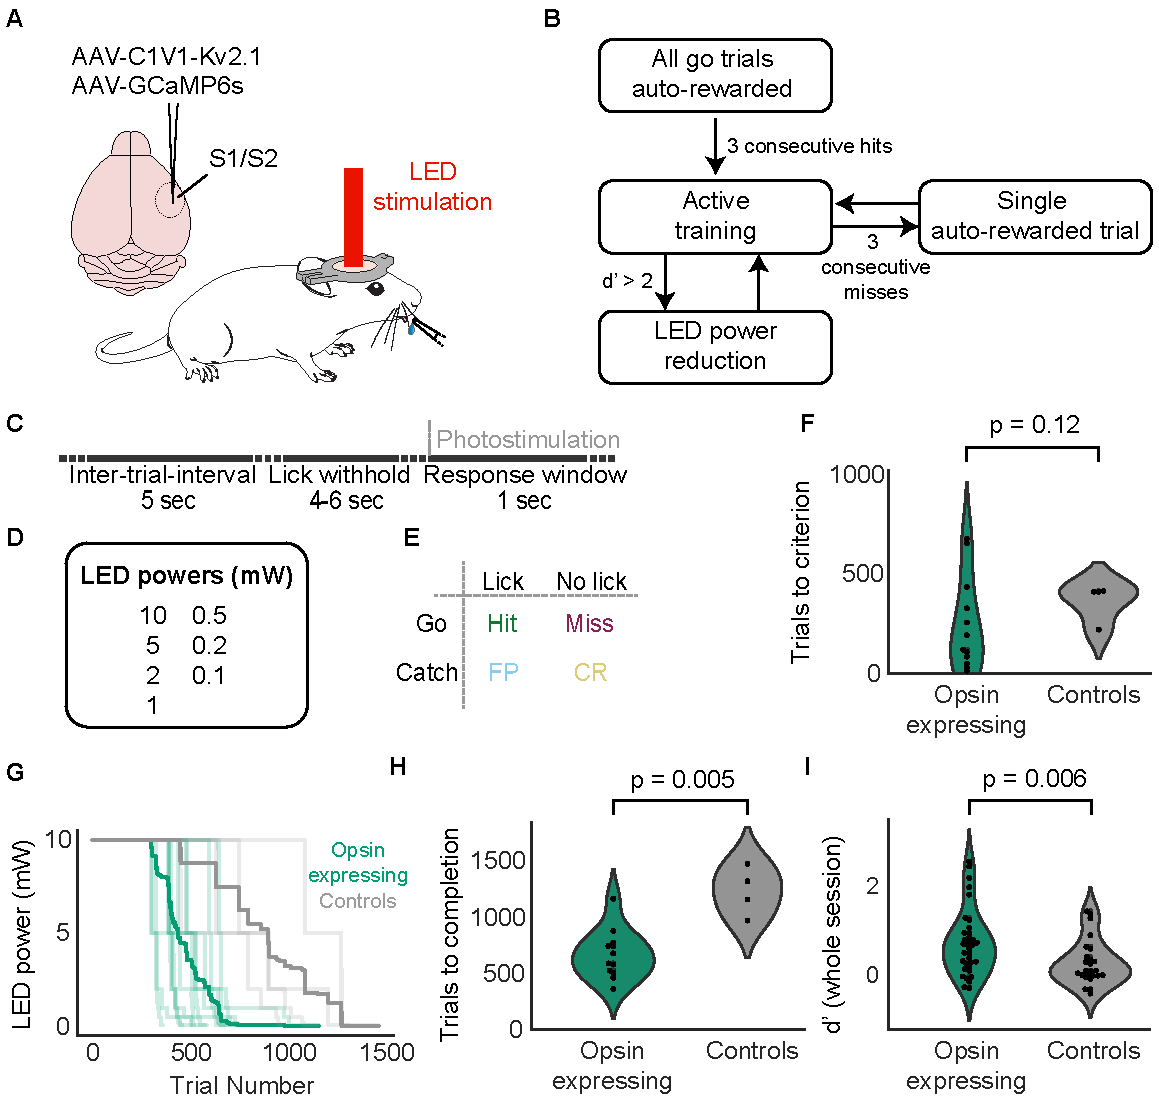
\includegraphics[scale=0.75]{figures/1-photon-behaviour.pdf}
\caption[\textbf{One-photon behavioural training.}]{
\textbf{One-photon behavioural training.}
\textbf{(A)} Schematic of the behavioural training setup. \textit{Left:} Viral injection performed in opsin expressing mice. \textit{Right:} Mice were headfixed and photostimulation was performed with an LED. A lick spout was placed within reach of the tongue, through which the animal reported perception of photostimulation by licking and received a water reward. \textbf{(B)} Steps in the fully automated training protocol. \textbf{(C)} Temporal structure of a single trial.  \textbf{(D)} LED powers used in the training. Mice started on 10 mW and were sequentially stepped down until they completed the task at 0.1 mW.  \textbf{(E)} Behavioral response matrix showing possible trial outcomes. \textbf{(F)} Number of trials required for mice to reach criterion (three consecutive hit trials) and complete the first stage of the task. Each point shows an individual mouse. \textbf{(G)} Ladder plot showing the LED power delivered to each mouse after a given number of trials. Thin transparent lines show individual mice and thick opaque lines show the average of the cohort. Mice were removed from the average calculation once they completed the task. Mice understood the task quicker if their ladder reached lower power levels after fewer trials. \textbf{(H)} Number of trials to complete the task for opsin expressing and control mice. Each point is an individual mouse. \textbf{(I)} d' across the whole session (for all power levels). Each point is an individual session.
} 
\label{fig:1-photon-behaviour}
\end{figure}

\section{Two-photon photostimulation}

Animals that had completed the one-photon task to the lowest power level were transitioned to two-photon photostimulation driven training. Mice were headfixed and an objective lens was placed, immersed in water, over the cranial window. The same objective lens was used to deliver two-photon photostimulation and perform two-photon calcium imaging (Figure \ref{fig:2-photon-behaviour}A) (see next section). The structure of the two-photon task is broadly the same as the one-photon (Figure \ref{fig:2-photon-behaviour}D,E). However, on go trials, we directly targeted photoresponsive S1 neurons with two photon photostimulation (see next section). In addition, on catch trials, although we did not deliver photostimulating light to the brain, we moved all optical components to mimic the auditory component of go trials, meaning the animal could not perform the task from auditory queues alone. Mice were only auto-rewarded for a single trial if they recorded three consecutive miss trials. Photoresponsive S1 neurons were identified before the onset of behaviour, by photostimulating all opsin expressing neurons, in groups of 20, to find cells responsive to photostimulation.

Mice began on a version of the task with two trial types, where go and catch trials were initiated with equal probability. On all go trials, 150 S1 neurons were photostimulated (Figure \ref{fig:2-photon-behaviour}B). Once mice achieved a d' > 1.5 across the entire session, they were transferred to the main version of the task, which generated the data included in all further plots.

The main version of the task introduced a third trial type, not present for initial training. Between 5 and 50 photoresponsive S1 neurons were stimulated on this trial type (Figure \ref{fig:2-photon-behaviour}C) (see materials and methods). The behaviour of an animal on a single session is shown in Figure \ref{fig:2-photon-behaviour}F. The lick raster indicates more reliable licking behaviour and a greater propensity to score a hit trial, when a greater number of neurons were stimulated.

The number and identity of cells stimulated was varied randomly on a trial by trial basis (see materials and methods), generating a psychometric curve (Figure \ref{fig:2-photon-behaviour}G) which demonstrates that stimulating a greater number of neurons more robustly drove licking behaviour, and that the inflection point of the psychometric curve fit across all sessions (N=10) is 23 neurons (95\% CI: 19 28), in accordance with previously published findings \cite{dalgleish_how_2020}. Therefore, by varying the identity and number of cells stimulated trial by trial, we delivered stimuli spanning the perceptual threshold of the animal, and ensured that the animal detects activity across the recorded population of S1 neurons rather than overtraining mice to report activity in a few specific neurons.

\begin{figure}[h]
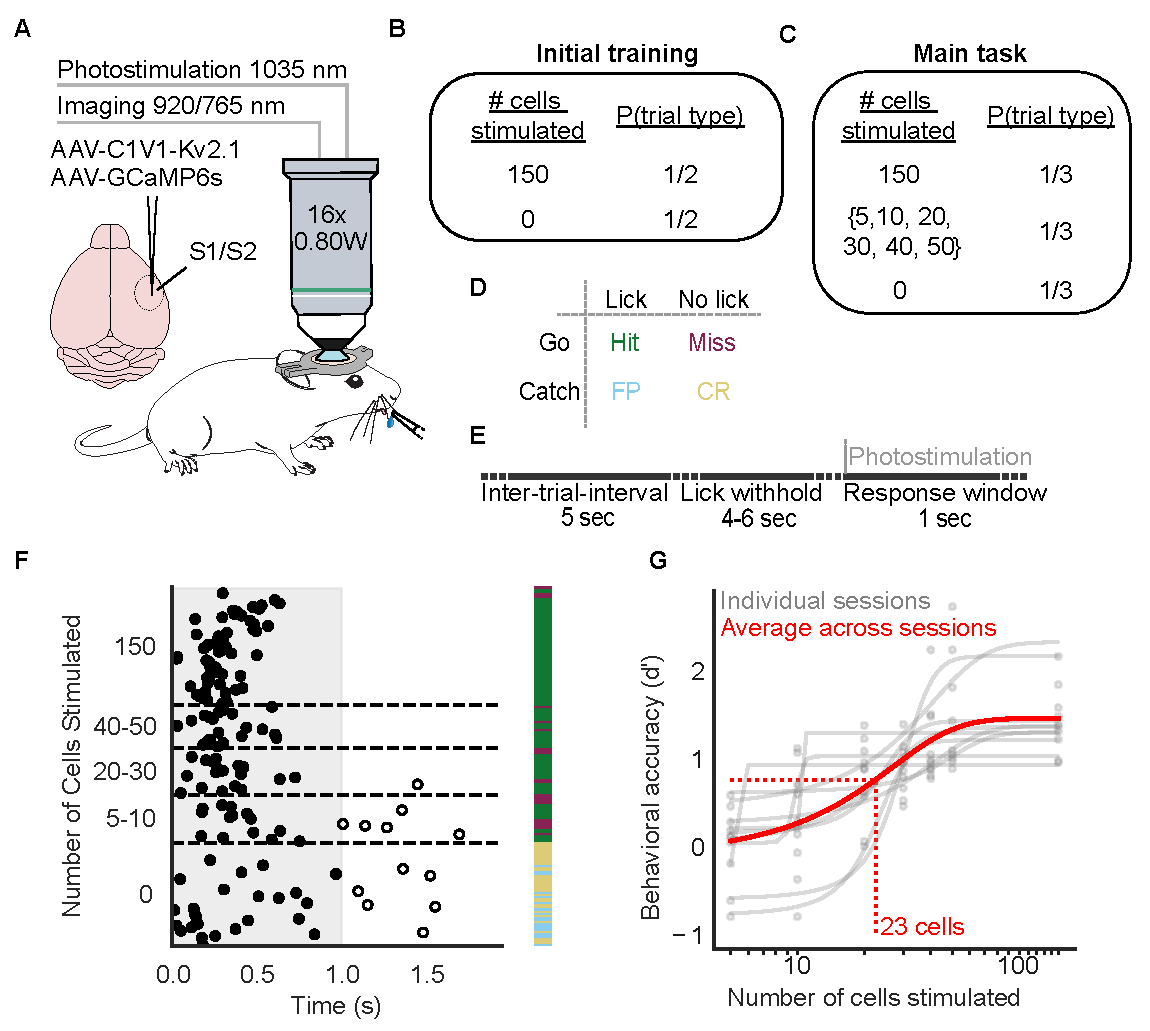
\includegraphics[scale=0.78]{figures/2-photon-behaviour.pdf}
\caption[\textbf{Two-photon behavioural training.}]{
\textbf{Two-photon behavioural training.}
\textbf{(A)} Schematic of experimental setup. \textit{Left}: viral strategy for expression of GCaMP6s and C1V1-KV2.1-mScarlet in S1 and S2.  \textit{Right}: mice with a cranial window installed over S1 and S2 were headfixed under a two-photon microscope. A lick spout was placed within reach of the tongue, through which the animal reported perception of photostimulation by licking and received a water reward. \textbf{(B)} Trial types for the initial stage of two-photon photostimulation training. \textbf{(C)} Trial types for the main task.  \textbf{(D)} Behavioral response matrix, the colour code matches that in F. \textbf{(E)} Timing of a single behavioral trial. \textbf{(F)} Example lick raster from a single session sorted by number of cells stimulated and by time within each bin. Each row of the plot shows the first lick within an individual trial. Filled circles are licks occurring within the response window, open circles are licks occurring after the response window closes. The colourbar shows the outcome of the trial as defined in the behavioral response matrix. \textbf{(G)} Psychometric curves showing behavioral performance (d’) as a function of the number of cells photostimulated. Each grey point is the d’ computed for a given number of cells stimulated for an individual session and each grey line is a logistic function fit for an individual session. The red solid line shows the fit for all data points across all sessions (N=10 sessions; N = 5 mice). The red dashed line shows the inflection point from the fit across all sessions. 
} 
\label{fig:2-photon-behaviour}
\end{figure}

In sum, this chapter demonstrates that I, alongside my colleagues, was able to develop a preparation in which experimentally controlled neural activity causally drove behaviour. Progression through the stages of training was automated, maximising repeatability and minimising human intervention. As explored in the next sections, this behavioural framework means that neural activity, causally underpinning behaviour, can be recorded, with single cell resolution, both locally and after propagation downstream.
\chapter{\label{res2}All-optical control of neural circuits across brain regions}

\minitoc

As referenced in the previous section on behaviour, we employed an "all-optical" approach, using light to both record neural activity and experimentally manipulate it, thus driving behaviour. This approach has previously been implemented to study individual brain regions \cite{dalgleish_how_2020, gill_precise_2020, russell_influence_2019, daie_targeted_2021, marshel_cortical_2019}, however here we adapted previously established all-optical procedures to study multiple brain regions, and how activity propagates between them to guide behaviour. 

\section{Localisation of S1 and S2}

To achieve this, we developed a preparation whereby activity in two brain regions (S1 and S2) was recorded simultaneously, while photostimulation was targeted to S1. To read and write neural activity, we expressed the genetically encoded calcium indicator GCaMP6s \cite{chen_ultrasensitive_2013} and the somatically targeted, red-shifted opsin C1V1-Kv2.1 \cite{yizhar_neocortical_2011, chettih_single-neuron_2019} in layer 2/3 across both S1 and S2. A cranial window was implanted to enable optical access to both regions simultaneously. We localised S1 and S2 by performing wide-field calcium imaging during deflection of individual whiskers (Figure \ref{fig:widefield}; methods). We stimulated whiskers individually (Figure \ref{fig:widefield}A), recording bulk calcium activity, and thus localising the somatotopic representation of the whisker pad indicative of S1 and S2 (Figure \ref{fig:widefield}B-E). Mice were only trained on behavioural tasks if they expressed opsin in S1 and calcium indicator in S1 and S2. In subsequent all-optical experiments, a field of view was selected which spanned multiple barrels of the a, b and c row both in S1 and S2 (Figure \ref{fig:widefield}B).

\begin{figure}[h]
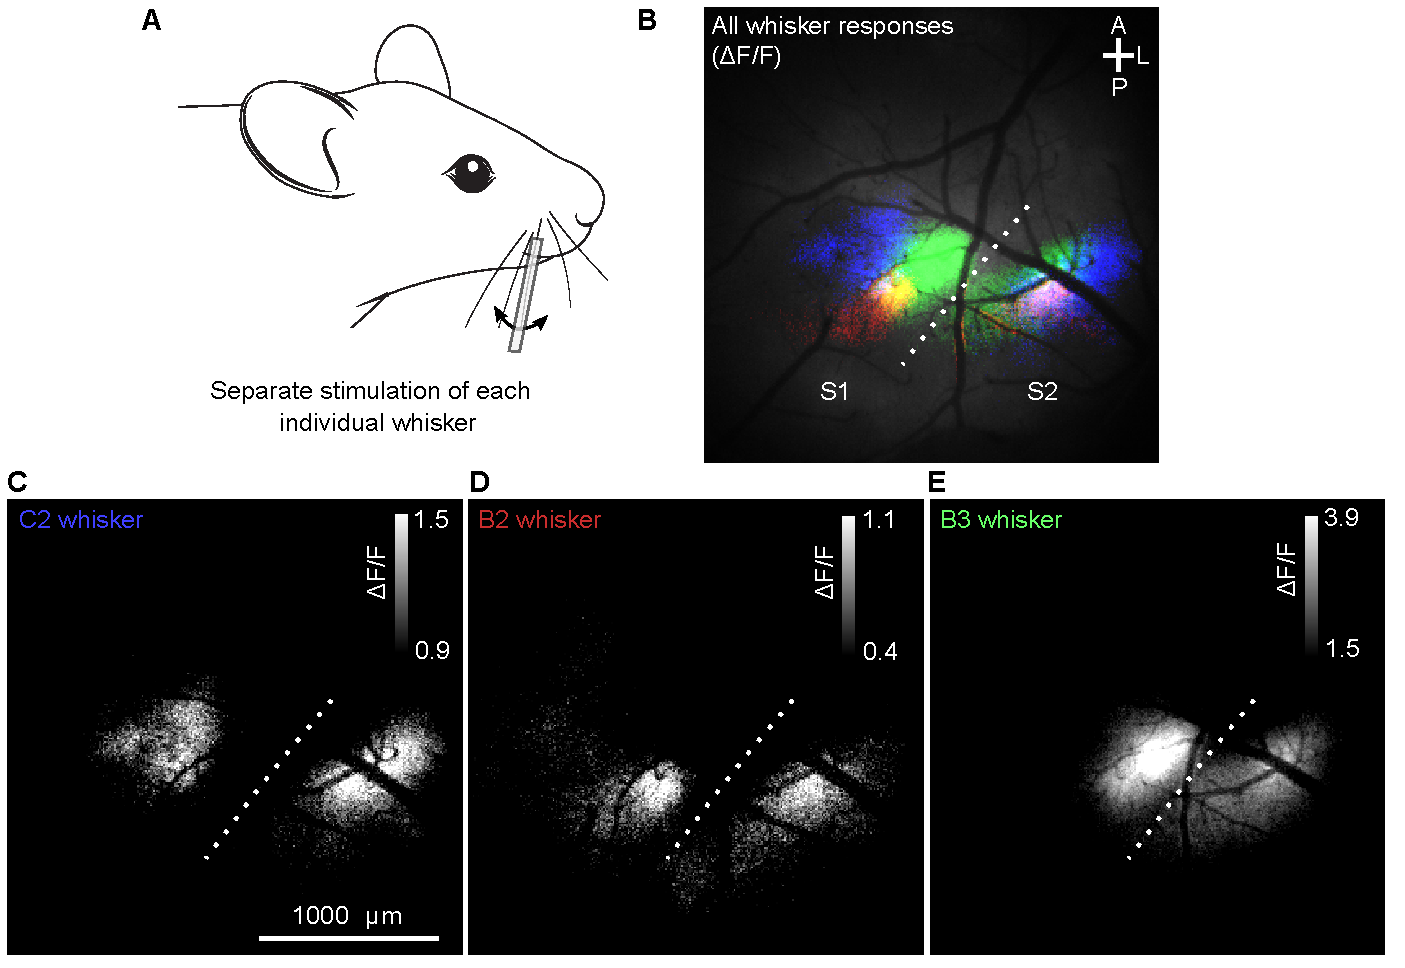
\includegraphics[scale=0.62]{figures/widefield-localisation.pdf}
\caption[\textbf{Widefield localisation of S1 and S2}]{
\textbf{Widefield localisation of S1 and S2}. \textbf{(A)} Individual whiskers of head-fixed mice were threaded into a capillary and deflected to elicit a neural response in the corresponding barrel. \textbf{(B)} Composite image showing a map of the barrel fields spanning S1 and S2 for an example mouse. \textbf{(C)} Trial averaged $\Delta$F/F responses from bulk widefield calcium imaging, across S1 and S2, following stimulation of the C2 whisker. \textbf{(D)} As C but for the B2 whisker. \textbf{(E)} As C but for the B3 whisker.
} 
\label{fig:widefield}
\end{figure}

\section{Simultaneous two-photon calcium imaging and photostimulation}

To read and write neural activity \textit{in vivo} across brain regions in a behaving animal, we employed a microscope, based on previous designs \cite{packer_simultaneous_2015}, adapted to perform two-photon calcium imaging of neural activity across a large field of view (1.35 mm diameter), while performing two-photon photostimulation of S1 neurons. As outlined in the previous section, mice expressing a calcium indicator and an opsin were head-fixed and the objective lens of the microscope was placed directly over their cranial window which spanned S1 and S2. 

Calcium imaging was performed with a resonant scanning system (Figure \ref{fig:all-optical}A), scanning at 30 Hz, to excite and image the genetically encoded calcium indicator GCaMP6s \cite{chen_behaviour-dependent_2013}. Spikes inferred from the slow ‘ultrasensitive’ variants of GCaMP have been shown to have correlations of >0.85 with ground truth spike trains \cite{friedrich_fast_2017}.

To photoactivate groups of cells simultaneously, we used a microscope with
a spatial light modulator (SLM) incorporated into the beam path of a laser capable of
two-photon excitation (Figure \ref{fig:all-optical}A). The SLM contains a reflective liquid crystal layer which acts as a two-dimensional diffraction grating, and thus can be used holographically to target multiple beamlets of light to arbitrary, user-defined points in space. This is demonstrated in Figure \ref{fig:all-optical}B in which fluorescence generated from 54 simultaneously generated beamlets was imaged on a wide-field camera.

The spatial resolution of an optical system is generally quantified using the point-spread function (PSF). In relation to imaging, this defines the smallest object that can be visualised, as the recorded image results from the convolution of the actual object and the PSF. The resolution of a two-photon imaging system is conventionally defined as the full width half max (FWHM) of the PSF and is usually degraded most in the axial dimension \cite{shaw_point-spread_1991}. The PSF can be recorded by imaging a sub-resolution fluorescence  source. The axial resolution for the resonant imaging system is shown in Figure \ref{fig:all-optical}C \textit{left}, generated by taking a "z-stack" to create a 3-dimensional image of the sub-resolution source from two-dimensional images taken at different focal depths. The PSF profile was then fit with a Gaussian function from the axial fluorescence intensity profile of the source, yielding a FWHM of 2.99 $\mu$m. This process can be repeated with the photostimulation beam, reflected off the SLM, to generate an image of a PSF describing the profile of the photostimulation beamlet on the sample, thus quantifying the resolution of the photostimulation system (Figure \ref{fig:all-optical}C right, FWHM = 19.8 $\mu$m). These two PSFs demonstrate that theoretically our microscope is able to read and write activity in individual neurons.

A proof-of-principle example of how two-photon calcium imaging and optogenetics can be used to read and write neural activity is shown in Figures \ref{fig:all-optical}D and E. Figure \ref{fig:all-optical}D shows calcium activity from five example neurons, recorded through fluorescence imaging of GCaMP6s, a surrogate for spikes \cite{chen_ultrasensitive_2013, huang_relationship_2021, grienberger_imaging_2012, packer_simultaneous_2015, stosiek_vivo_2003}. Figure \ref{fig:all-optical}E demonstrates how neural activity can be injected into individual neurons expressing opsin, without driving spikes in neighbouring opsin-expressing neurons. Only the  cell targeted with two-photon photostimulation exhibits a clear increase in fluorescence locked  temporally to the stimulus onset.

\begin{figure}[!h]
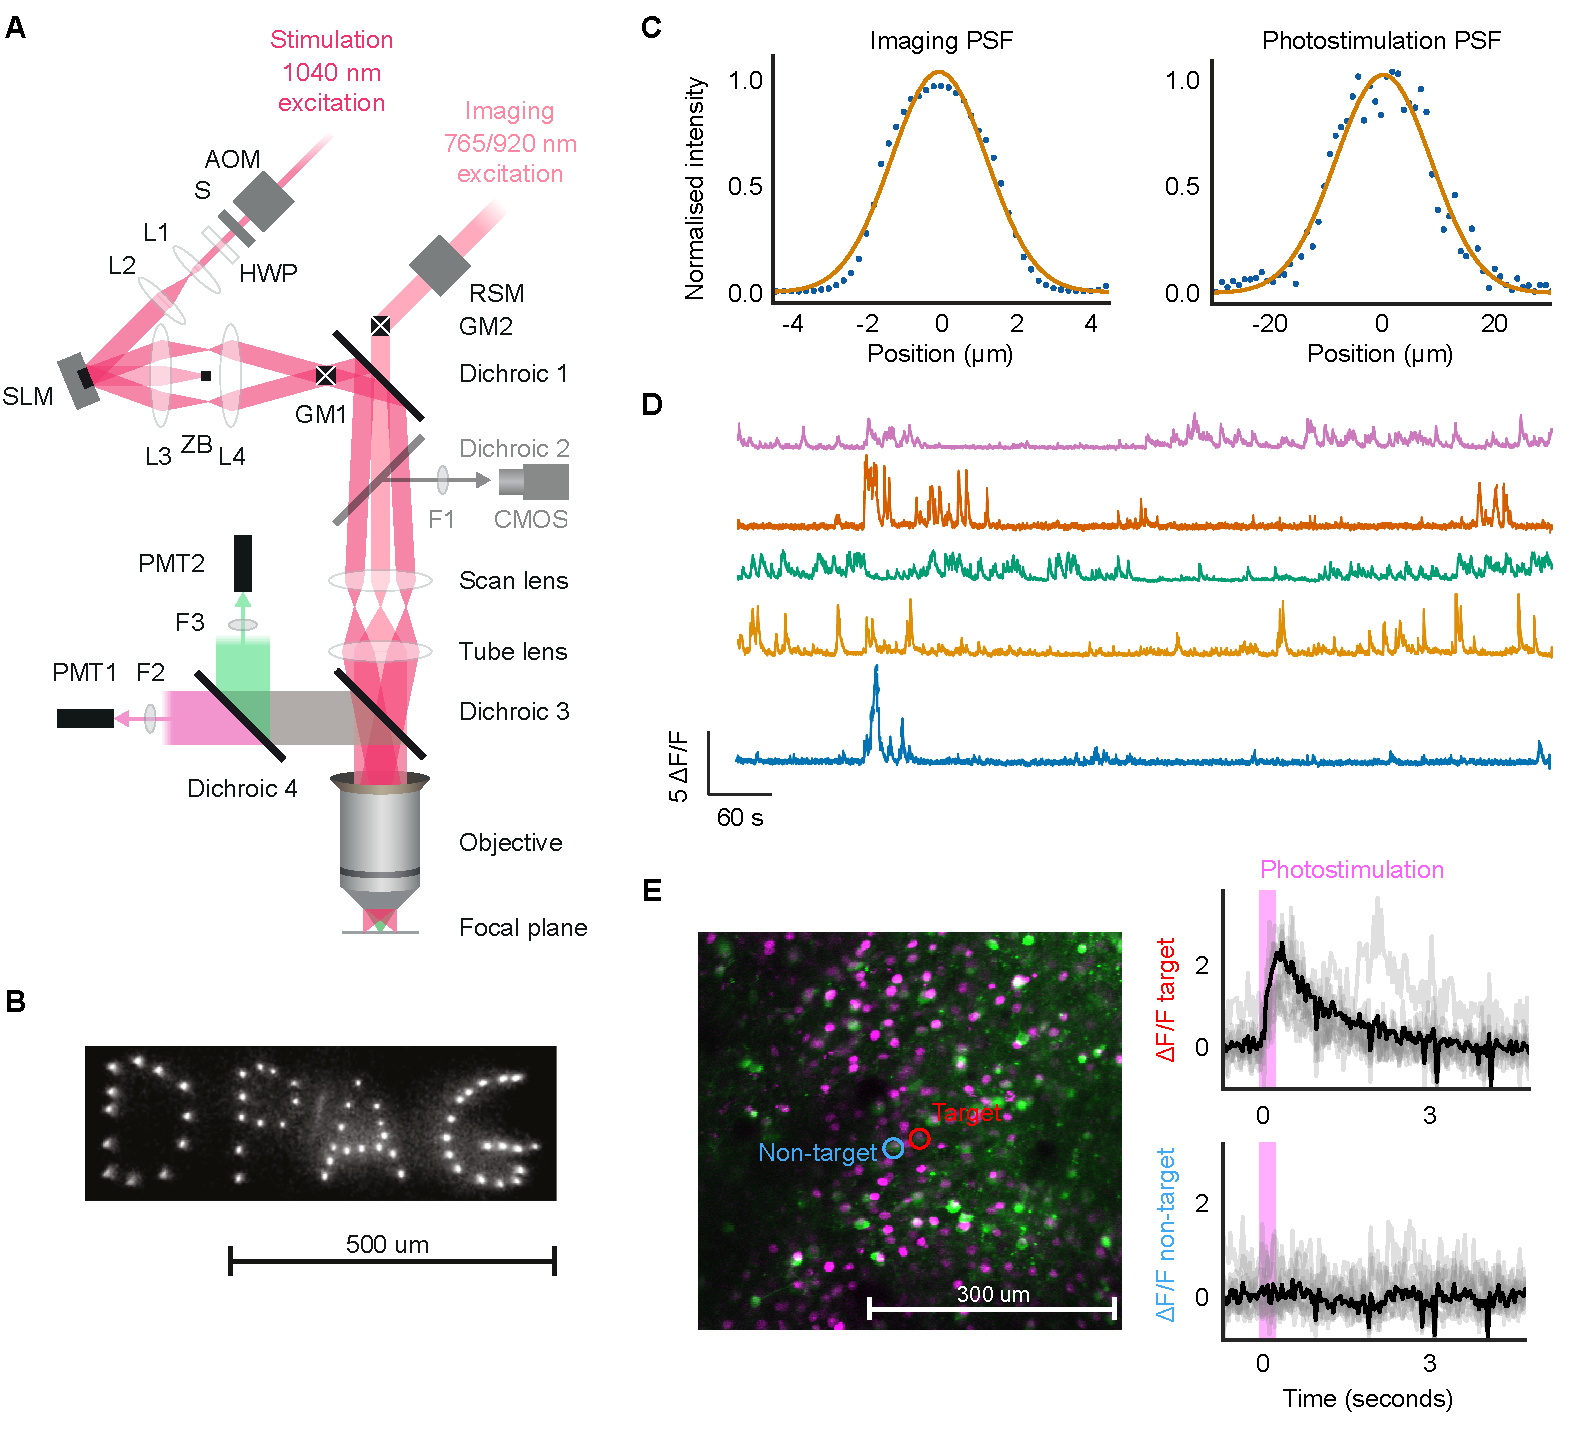
\includegraphics[scale=0.567]{figures/2p_imaging+photostim.pdf}
\caption[\textbf{Two-photon calcium imaging and photostimulation}]{
\textbf{Two-photon calcium imaging and photostimulation. (A)} Layout of the all-optical beam path. AOM, acousto-optic modulator; S, shutter; HWP, half-wave plate; L1-4, lenses; SLM, spatial light modulator; ZB, zero order block; GM1, GM2, galvanometers; RSM, resonant scanning module; F1-3, filters; PMT1, PMT2, photomultiplier tubes. Figure adapted from \cite{packer_simultaneous_2015}. \textbf{(B)} Beamlets generated by splitting the photostimulation beam with the SLM. For display purposes beamlets were imaged on a fluorescent plastic slide using a widefield camera (DPAG = department of physiology, anatomy and genetics). \textbf{(C)} \textit{Left}: Axial PSF of the resonant imaging system (FWHM = 2.99 um). \textit{Right}: Axial PSF of the photostimulation system (FWHM
= 19.8 um). \textbf{(D)} Example calcium traces from 5 neurons imaged at 30 Hz. Traces were smoothed for display with a running mean of 3 frames. \textbf{(E)} \textit{Left}: Example field of view of a mouse expressing the calcium indicator GCaMP6s (green) and the opsin ST-ChroME \cite{mardinly_precise_2018} (magenta) (used only for this calibration experiment). The cell targeted for two-photon holographic photostimulation is highlighted in red. \textit{Right}: Fluorescence traces resulting from 10 trials of targeted photostimulation. Individual trials are shown in grey and the mean response across all trials is shown in black. 
} 
\label{fig:all-optical}
\end{figure}

While these proof of principal experiments prove that we can photostimulate and record from individual neurons, the behavioural experiment requires that we photostimulate groups of multiple S1 neurons, varying on a trial by trial basis, while imaging across S1 and S2. The principles behind this are outlined in figure \ref{fig:s1s2}. Mice expressing the calcium indictor GCaMP6s \cite{chen_ultrasensitive_2013} and the red-shifted soma-targetted opsin C1V1-kv2.1 \cite{yizhar_neocortical_2011, chettih_single-neuron_2019} were headfixed under the objective of the beam path outlined in Figure \ref{fig:all-optical}. 

A field of view was selected which spanned multiple barrels of the a, b and c row both in S1 and S2 (Figure \ref{fig:s1s2}B,C) which was small enough that we could image it with two-photon calcium imaging with single-cell resolution. Before the behavioural experiment, we photostimulated all opsin-expressing neurons in multiple small groups, to find cells responsive to photostimulation, with neurons within a 350 μm diameter stimulated simultaneously. Each group of neurons was photostimulated for 250 ms, with 5 ms between the stimulation of each group. Trial averaged, excitatory responses to this "pre-behaviour" photostimulation can be visualised as a stimulus triggered average image (see methods) in which responses were apparent in neurons proximal to the photostimulation beam (“targets”, defined as cells within 15 µm of the center of the beam) (Figure \ref{fig:all-optical}C; methods).

A demonstrative example of how multiple groups of neurons can be targeted in quick succession is shown in figure \ref{fig:s1s2}D. Phase masks are loaded onto the SLM, with a 5 ms inter-mask-interval, resulting in multiple beamlets of light targeted to individual cell soma. As shown in the STA images (methods) from the neural response generated by each of these masks, only cells directly under the photostimulation targets are activated by light. 

As discussed in the previous section, and methods, during behavioural training we targeted between 5 and 150 photoresponsive neurons on each go trial. Groups of between 5 and 50 neurons could be targeted simultaneously with a single phase mask. The cells comprising the groups were chosen randomly with replacement on a trial by trial basis. However our system does not have the photostimulation beam power or spatial range to stimulate 150 cells simultaneously. Hence this was achieved by stimulating 3 groups of 50 neurons sequentially, resulting in a total stimulation length of 750 ms. The trial-averaged responses of targeted and non-targeted cells, both in S1 and S2, during behaviour is shown for a single session in Figure \ref{fig:s1s2}E. A clear excitatory response is only observed, when averaging across trials, in targeted neurons. As the identity of targeted cells was varied trial to trial, the cells averaged to form the traces was not the same on every trial.

\begin{figure}[h]
\hspace*{-0.4in}
\includegraphics[scale=0.6]{figures/multiarea_ao.pdf}
\caption[\textbf{All-optical interrogation across brain regions}]{
\textbf{All-optical interrogation across brain regions (A)} Schematic of experimental setup. \textit{Left}: viral strategy for expression of GCaMP6s and C1V1-KV2.1-mScarlet in S1 and S2.  \textit{Right}: mice with a cranial window installed over S1 and S2 were headfixed under a two-photon microscope. A lick spout was placed within reach of the tongue, through which the animal reported perception of photostimulation by licking and received a water reward. \textbf{(B)} Example widefield calcium imaging field of view used to localise S1 and S2 by whisker stimulation. \textbf{(C)} STA image. Example two-photon calcium imaging field of view with photostimulation targets. The intensity of each pixel is proportional to the change in fluorescence intensity post-photostimulation compared to pre-photostimulation; bright pixels indicate a photostimulation-induced increase in calcium activity. Pixels are color-coded based on whether they were photostimulated simultaneously. Non-targeted cells, including those in S2 are not visible when averaging across a single stimulation group.
\textbf{(D)} Sequential photostimulation. An
automated protocol was used to target groups of cells for simultaneous stimulation. Groups
were stimulated for 250 ms with a 5 ms inter-group-interval. 10 trials of stimulation were
performed. \textit{Top}: Phase masks loaded onto the SLM to generate targets. \textit{Bottom}: STA images (methods). The pixel intensity of the images shows the change in fluorescence compared to baseline, averaged across trials, following photostimulation of the targets (yellow circles). \textbf{(E)} Example activity responses to photostimulation in a single behavioural session. Blue shows the response to photostimulation of cells directly targeted with light, averaged across cells and across trials. Orange and green show the response of cells not directly targeted in S1 and S2 respectively. Only trials in which photostimulation was delivered were included and data were baselined to the pre-stimulus mean on a cell-wise and trial-wise basis before averaging. Data are blanked while the photostimulation laser was on (pink bar) as this causes a large artifact unrelated to neural activity.
} 
\label{fig:s1s2}
\end{figure}

In sum, this chapter demonstrates that I, alongside my colleagues, developed methodologies that allowed all-optical techniques to be applied across multiple brain regions. This tool can then be combined with the behavioural paradigm outlined in the previous section to study neural activity, causal in behaviour as it propagates between brain regions.
\chapter{\label{res3}Statistical modelling of evoked neural activity
}

\minitoc

To understand how neural activity is propagated between brain regions in order to guide behaviour, we used the all-optical methodology outlined in the previous two sections to compare the neural response during reported and non-reported stimuli (hit and miss trials respectively), both in the directly stimulated region (S1) and an anatomically connected downstream region (S2). 

\section{The structure of evoked activity in S1 and S2}

To display visually the response of individual S1 and S2 neurons to hit and miss trials, we plotted their trial averaged responses as raster plots (Figure \ref{fig:basic-analysis}A; Figures \ref{fig:supp2},\ref{fig:supp3}). Qualitatively, hit trials elicit a diverse array of excitatory and inhibitory responses both in S1 and S2, whereas both excitatory and inhibitory responses were less obvious on miss trials. Excited and inhibited cells are also observed in ‘reward only’ trials (methods) in which reward was delivered in the absence of photostimulation, however the population response is less pronounced compared to hit trials, indicating that the response to reported stimulation is not just explained by neural activity driven by reward (Figure \ref{fig:basic-analysis}A; Figures \ref{fig:supp2},\ref{fig:supp3}). We find that hit trials elicit a significantly greater fraction of responsive cells in S1 compared to all other trial types, whereas in S2, hit trials elicited a significantly greater fraction of responsive cells only compared to correct rejection and reward only trials (p < 0.05, Bonferroni corrected). The fraction of responsive cells was greater in S2 compared to miss and false positive trials but this result was not significant (p > 0.05, Bonferroni corrected) (Figure \ref{fig:supp1}A). On a single cell level, we find individual neurons in S2 that are excited or inhibited in response to hit trials, but not miss or reward only, hinting that reported stimuli are propagated to single neurons in S2 (Figure \ref{fig:basic-analysis}B).

\begin{figure}[htbp]
\vspace*{-2.5cm}
\thisfloatpagestyle{empty}
\hspace*{-0.25in}
% \vspace*{-0.1in}
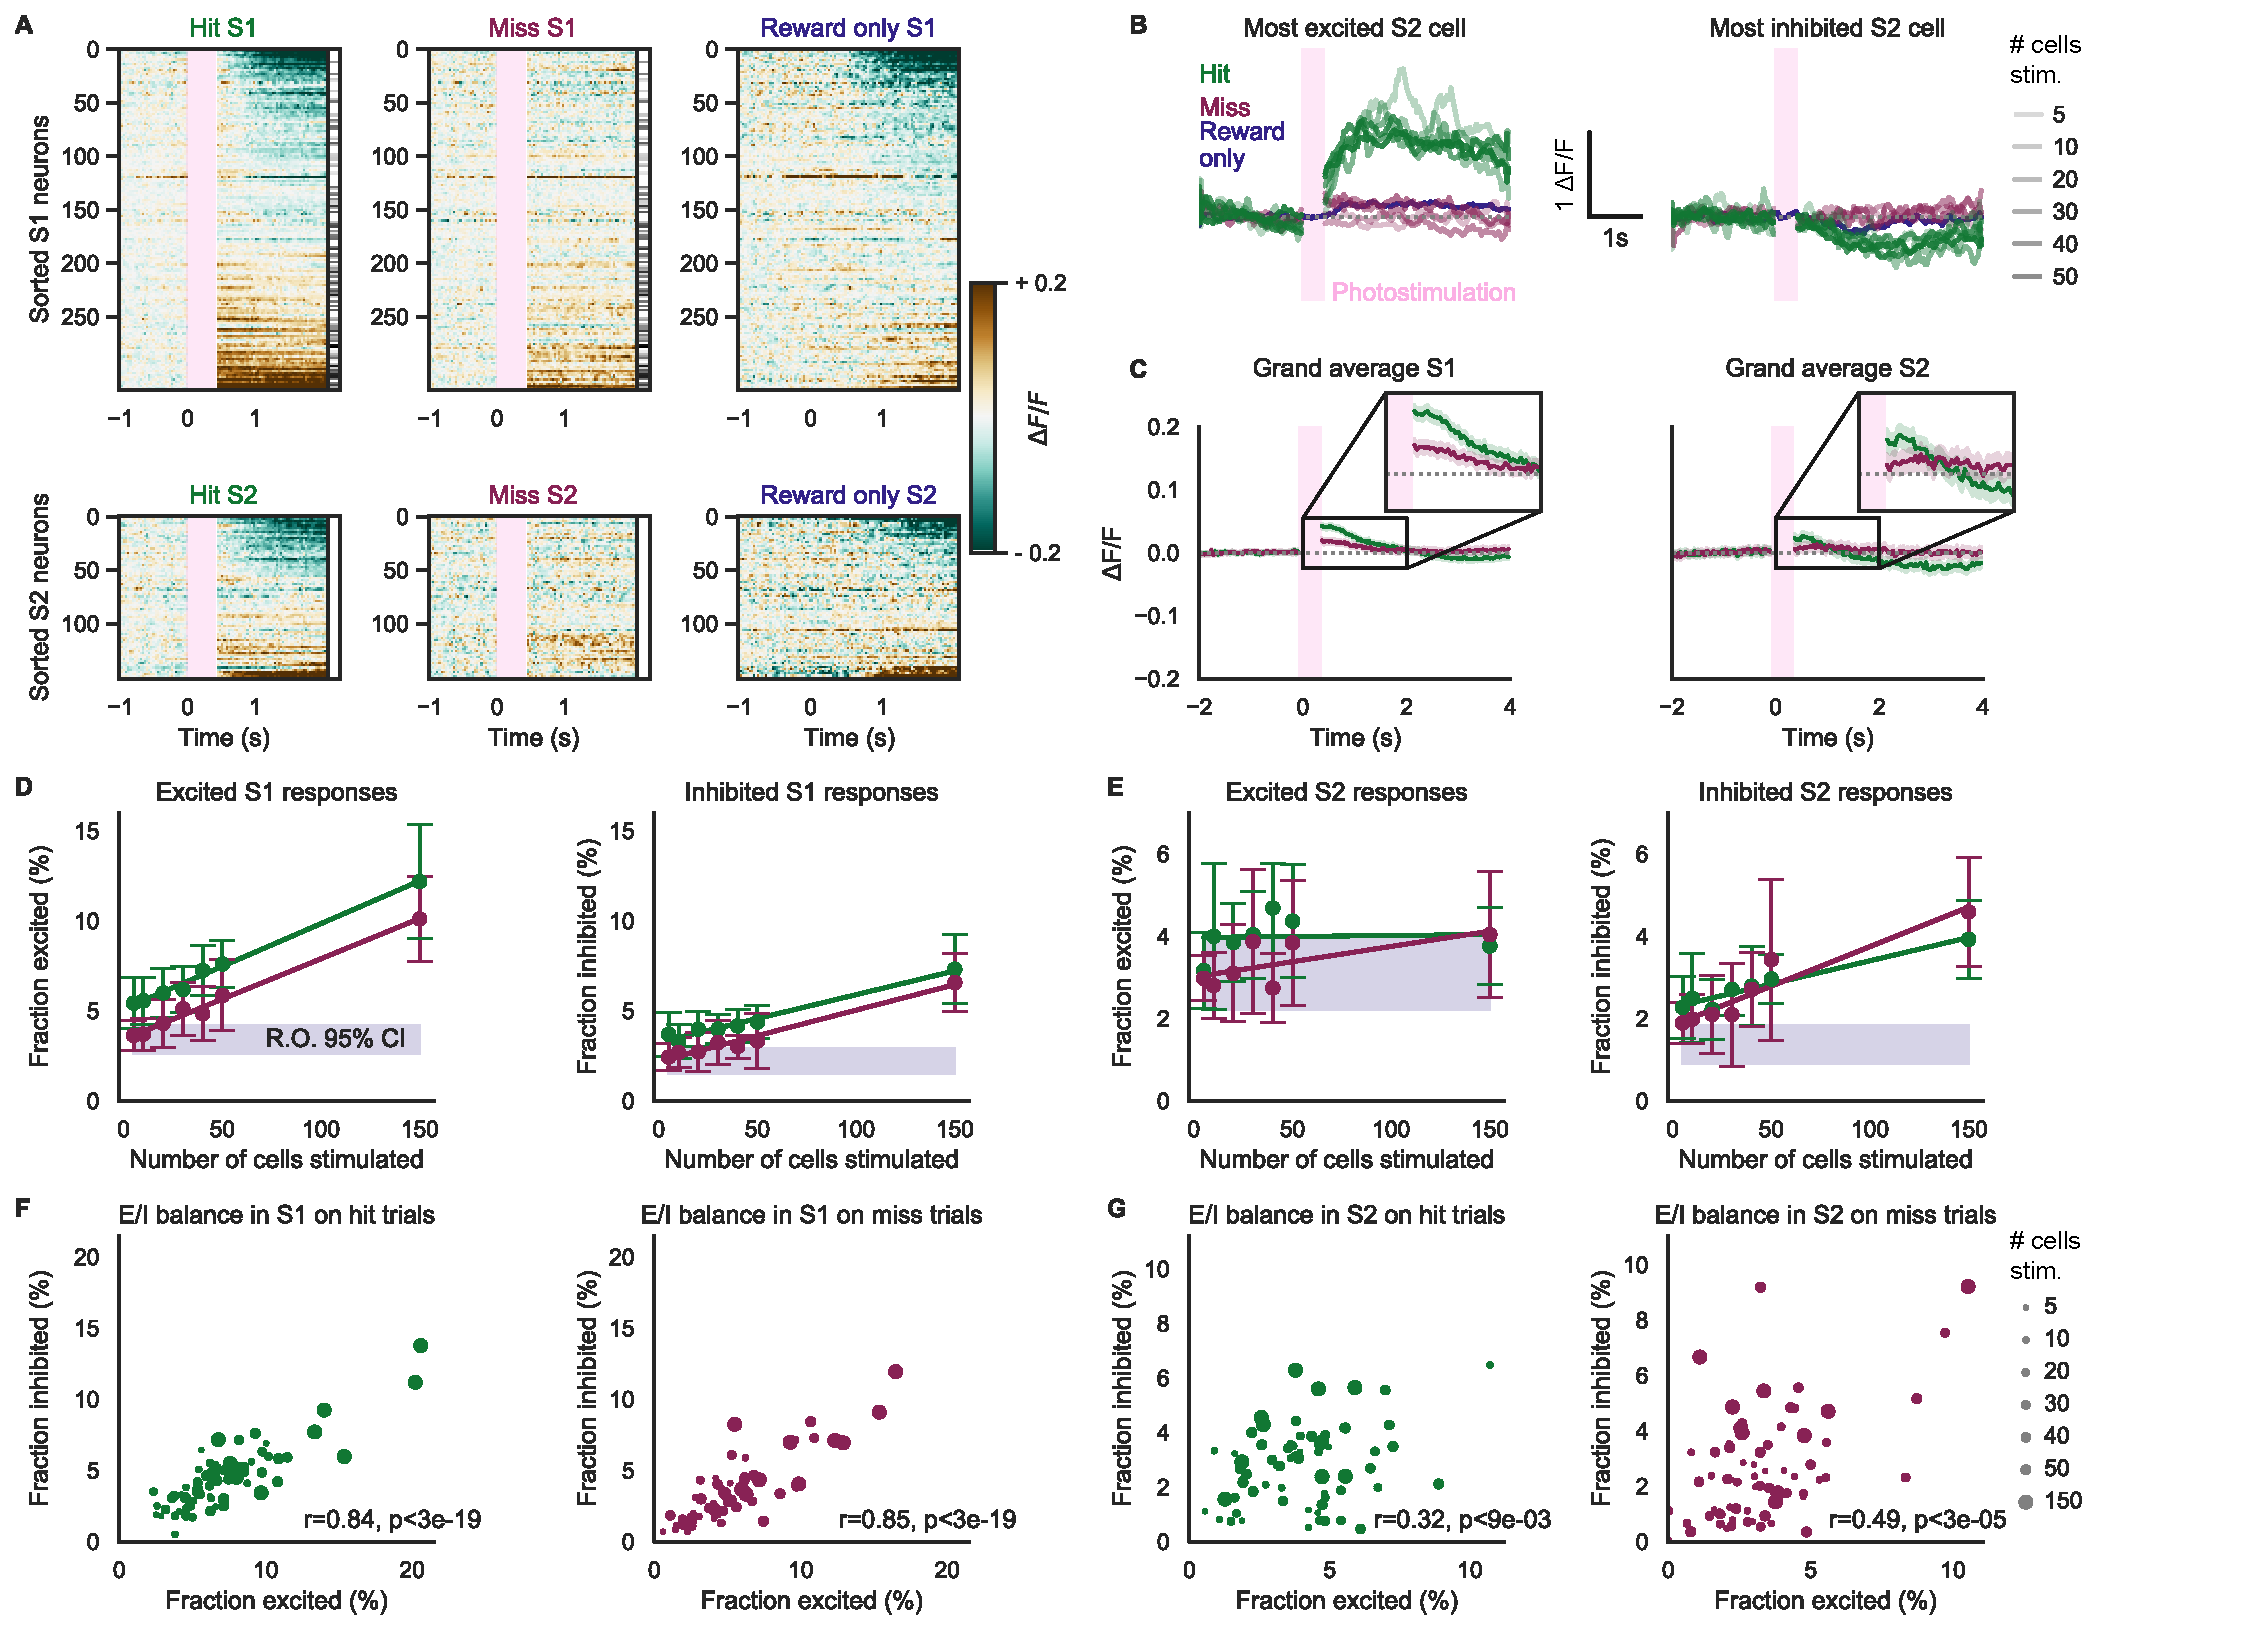
\includegraphics[scale=0.45]{figures/basic-analysis.pdf}
\caption[\textbf{Structure of evoked activity in S1 and S2}]{
\textbf{Structure of evoked activity in S1 and S2}. \textbf{(A)} Raster plots showing the trial averaged response to trial types (Left: hit, Middle: miss, Right: reward only) to photostimulation (pink vertical bar, hit/miss)  and/or reward (hit/reward only) of individual cells from a single session. Data were baselined to the pre-stimulus mean on a cell-wise basis before averaging. Cells are sorted by the pairwise correlation between their trial averaged responses across all three trial types (methods). A clear excitatory and inhibitory response is elicited in S1 and S2 on hit trials that cannot be solely attributed to reward. The intensity of the bar on the right hand side of the hit and miss rasters is proportional to the number of times each cell was directly targeted by the photostimulation beam. Trials in which 150 cells were stimulated were removed for display. Data are blanked while the photostimulation laser was on (pink bar). \textbf{(B)} \textit{Left}: Example S2 cell excited on hit trials (green) but showing no response to miss trials (red) or reward only trials (blue). Each line shows an individual trial. The transparency of the line indicates the number of cells stimulated in S1. Individual trials were baslined to the pre-stimulus mean. Right: Example S2 cell inhibited on hit trials. Trials in which 150 cells were stimulated were removed for display. \textbf{(C)} Average population response to hit and miss trials across all sessions. Traces are averaged across cells, trials and sessions for a given trial type. Individual trials were baselined to the pre-stimulus mean. Trials in which 150 cells were stimulated were removed for display. \textbf{(D)} Function mapping the response in S1 on hit and miss trials to the number of cells stimulated in S1. Left: The fraction of excited cells in S1 maps linearly to the number of cells photostimulated on both hit and miss trials. Right: The fraction of inhibited cells in S1 maps linearly to the number of cells photostimulated on both hit and miss trials. The shaded purple bar shows the fraction of excited or inhibited cells in S1 on reward only (R.O.) trials. \textbf{(E)} Function mapping the response in S2 on hit and miss trials to the number of cells stimulated in S1. Left: There is no relationship between the fraction of excited cells in S2 and the number of cells stimulated in S1 on hit trials or miss trials. The shaded purple bar shows the fraction of excited or inhibited cells in S2 on reward only trials. Right: The fraction of inhibited cells in S2 maps linearly to the number of cells photostimulated in S1 on both hit and miss trials. \textbf{(F)} Population E/I balance in S1 following photostimulation. The fraction of cells excited by photostimulation in S1 is highly correlated with the fraction of cells inhibited both on hit trials (left) and miss trials (right). The size of the circle indicates the number of cells photostimulated. \textbf{(G)} Population E/I balance in S2 following photostimulation in S1. The fraction of cells excited by photostimulation in S1 is significantly correlated with the fraction of cells inhibited both on hit trials (left) and miss trials (right). However the magnitude of the correlation is lower than in S1. The size of the circle indicates the number of cells photostimulated. 
} 
\label{fig:basic-analysis}
\end{figure}

Interestingly however, averaging responses across cells, trials and sessions reveals that hit trials elicit only a modest increase in population activity from baseline, immediately following stimulation, in S1 and S2, followed by a prolonged period of inhibition. Whereas the reward only condition exhibited a very different time course (Figure \ref{fig:basic-analysis}C; Figure \ref{fig:supp1}B,C). This hints that both brain regions exist in balanced regimes whereby excitation driven by photostimulation results in inhibition of roughly equal magnitude. Miss trials elicit excitation following photostimulation in S1, however this excitation is not observed as propagated activity in trial-and-cell-averaged responses downstream in S2 (Figure \ref{fig:basic-analysis}C). 


\begin{figure}[h]
\hspace*{-0.25in}
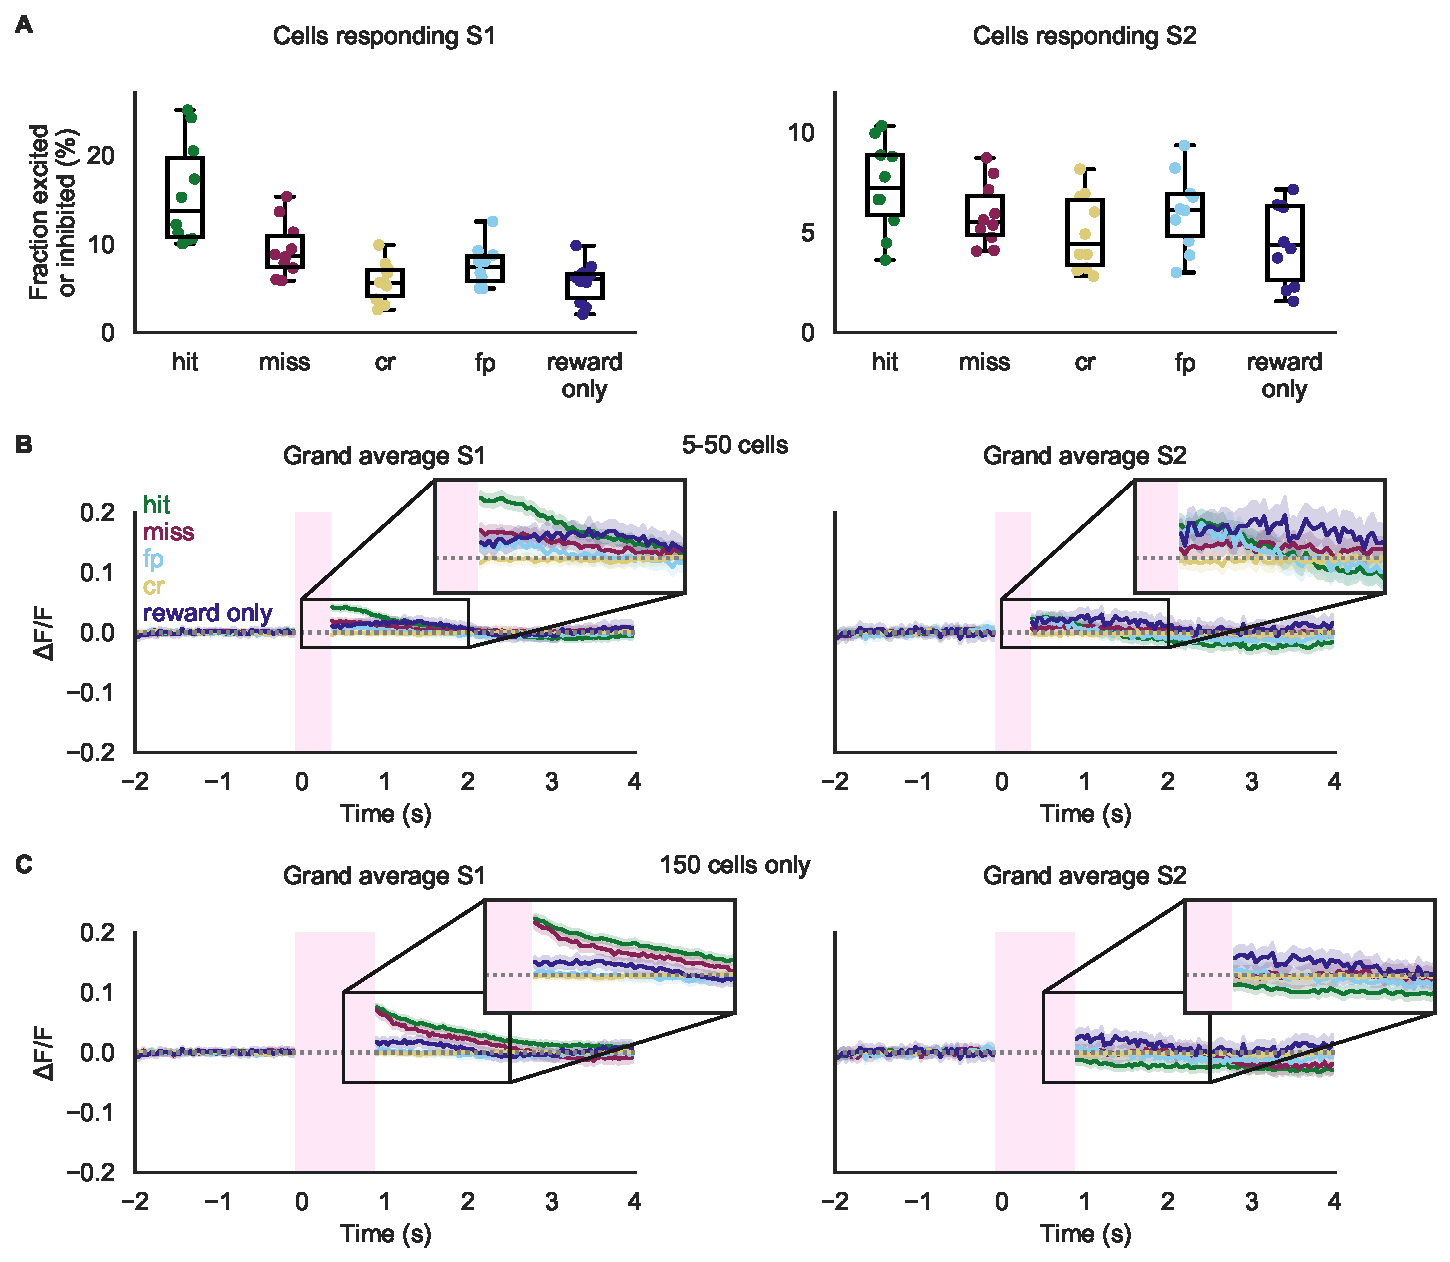
\includegraphics[scale=0.65]{figures/supplements/Supplementary_Figure1.pdf}
\caption[\textbf{Fraction of cells responding and grand average traces of all trial types in S1 and S2}]{\textbf{ Fraction of cells responding and grand average traces of all trial types in S1 and S2.
 (A)} The fraction of responsive cells (both excited and inhibited) on each trial type across all numbers of cells stimulated. \textbf{(B)} Average population response to all trial types across all sessions. Traces are averaged across cells, trials and sessions for a given trial type. Individual trials were baselined to the pre-stimulus mean. Trials in which 150 cells were stimulated were removed for display. \textbf{(C)} As above but including only trials in which 150 cells were stimulated. 
} 
\label{fig:supp1}
\end{figure}


We next compared how the percentage of excited or inhibited neurons, both locally in S1 and downstream in S2, scaled with the number of cells photostimulated in S1 and whether this differed between perceived and non-perceived stimuli (Figure \ref{fig:basic-analysis}D,E). As expected, stimulating more neurons in S1 excited a greater percentage of the population regardless of whether the stimulus was perceived (Figure \ref{fig:basic-analysis}D left)  (Pearson’s r = 0.62, p  = 1.8x10\textsuperscript{-8} hit trials; Pearson’s r = 0.65, p = 2.4x10\textsuperscript{-9} miss trials). We also find that the percentage of inhibited cells in S1 also scales linearly with the number of cells stimulated (Figure \ref{fig:basic-analysis}D right) (Pearson’s r = 0.55, p = 1.2x10\textsuperscript{-6} hit trials; Pearson’s r = 0.59, p = 1.4x10\textsuperscript{-7} miss trials). This indicates that excitatory photostimulation elicits a compensatory inhibitory response local to the stimulation. In S2, downstream of the stimulation, however the population response to increasing numbers of stimulated cells is more complex. We find no significant relationship between the percentage of excited cells in S2 and the number of stimulated cells in S1 on hit trials or miss trials, although the correlation is an order of magnitude greater on miss trials (Pearson’s r = 0.01, p = 0.9 hit trials; Pearson’s r = 0.17, p = 0.16 miss trials). However we find that the percentage of inhibited cells in S2 scales linearly with the number of stimulated cells in S1 both on hit and on miss trials (Figure \ref{fig:basic-analysis}E left, right) (Pearson’s r = 0.37, p = 0.002 hit trials; Pearson’s r = 0.45, p = 1.2x10\textsuperscript{-4} miss trials).

Next, we explicitly quantified the balance between excitation and inhibition (E/I) in both brain regions. We find robustly maintained E/I balance in S1 regardless of whether or not the stimulation was perceived, whereby the percentage of cells excited and inhibited is highly correlated (Figure \ref{fig:basic-analysis}F) (Pearson’s r = 0.84, p < 3x10\textsuperscript{-19} hit trials; Pearson’s r = 0.85, p < 3x10\textsuperscript{-19} miss trials). Downstream in S2, we also find E/I balance both on hit trials and miss trials, however the correlation is less strong than in S1, and is weaker on hit trials than miss trials (Figure \ref{fig:basic-analysis}G) (Pearson’s r = 0.32, p < 0.009 hit trials; Pearson’s r = 0.49, p < 3x10\textsuperscript{-5} miss trials). Taken together, we show that as activity is propagated away from its site of initiation, E/I balance persists but its strength is reduced. Additionally, perceived stimuli escape the balanced regime downstream to a greater extent than non-perceived stimuli as evidenced by the stronger correlation between the percentage of excited and inhibited cells on miss trials compared to hit trials. 


\begin{figure}[h]
\hspace*{-0.6in}
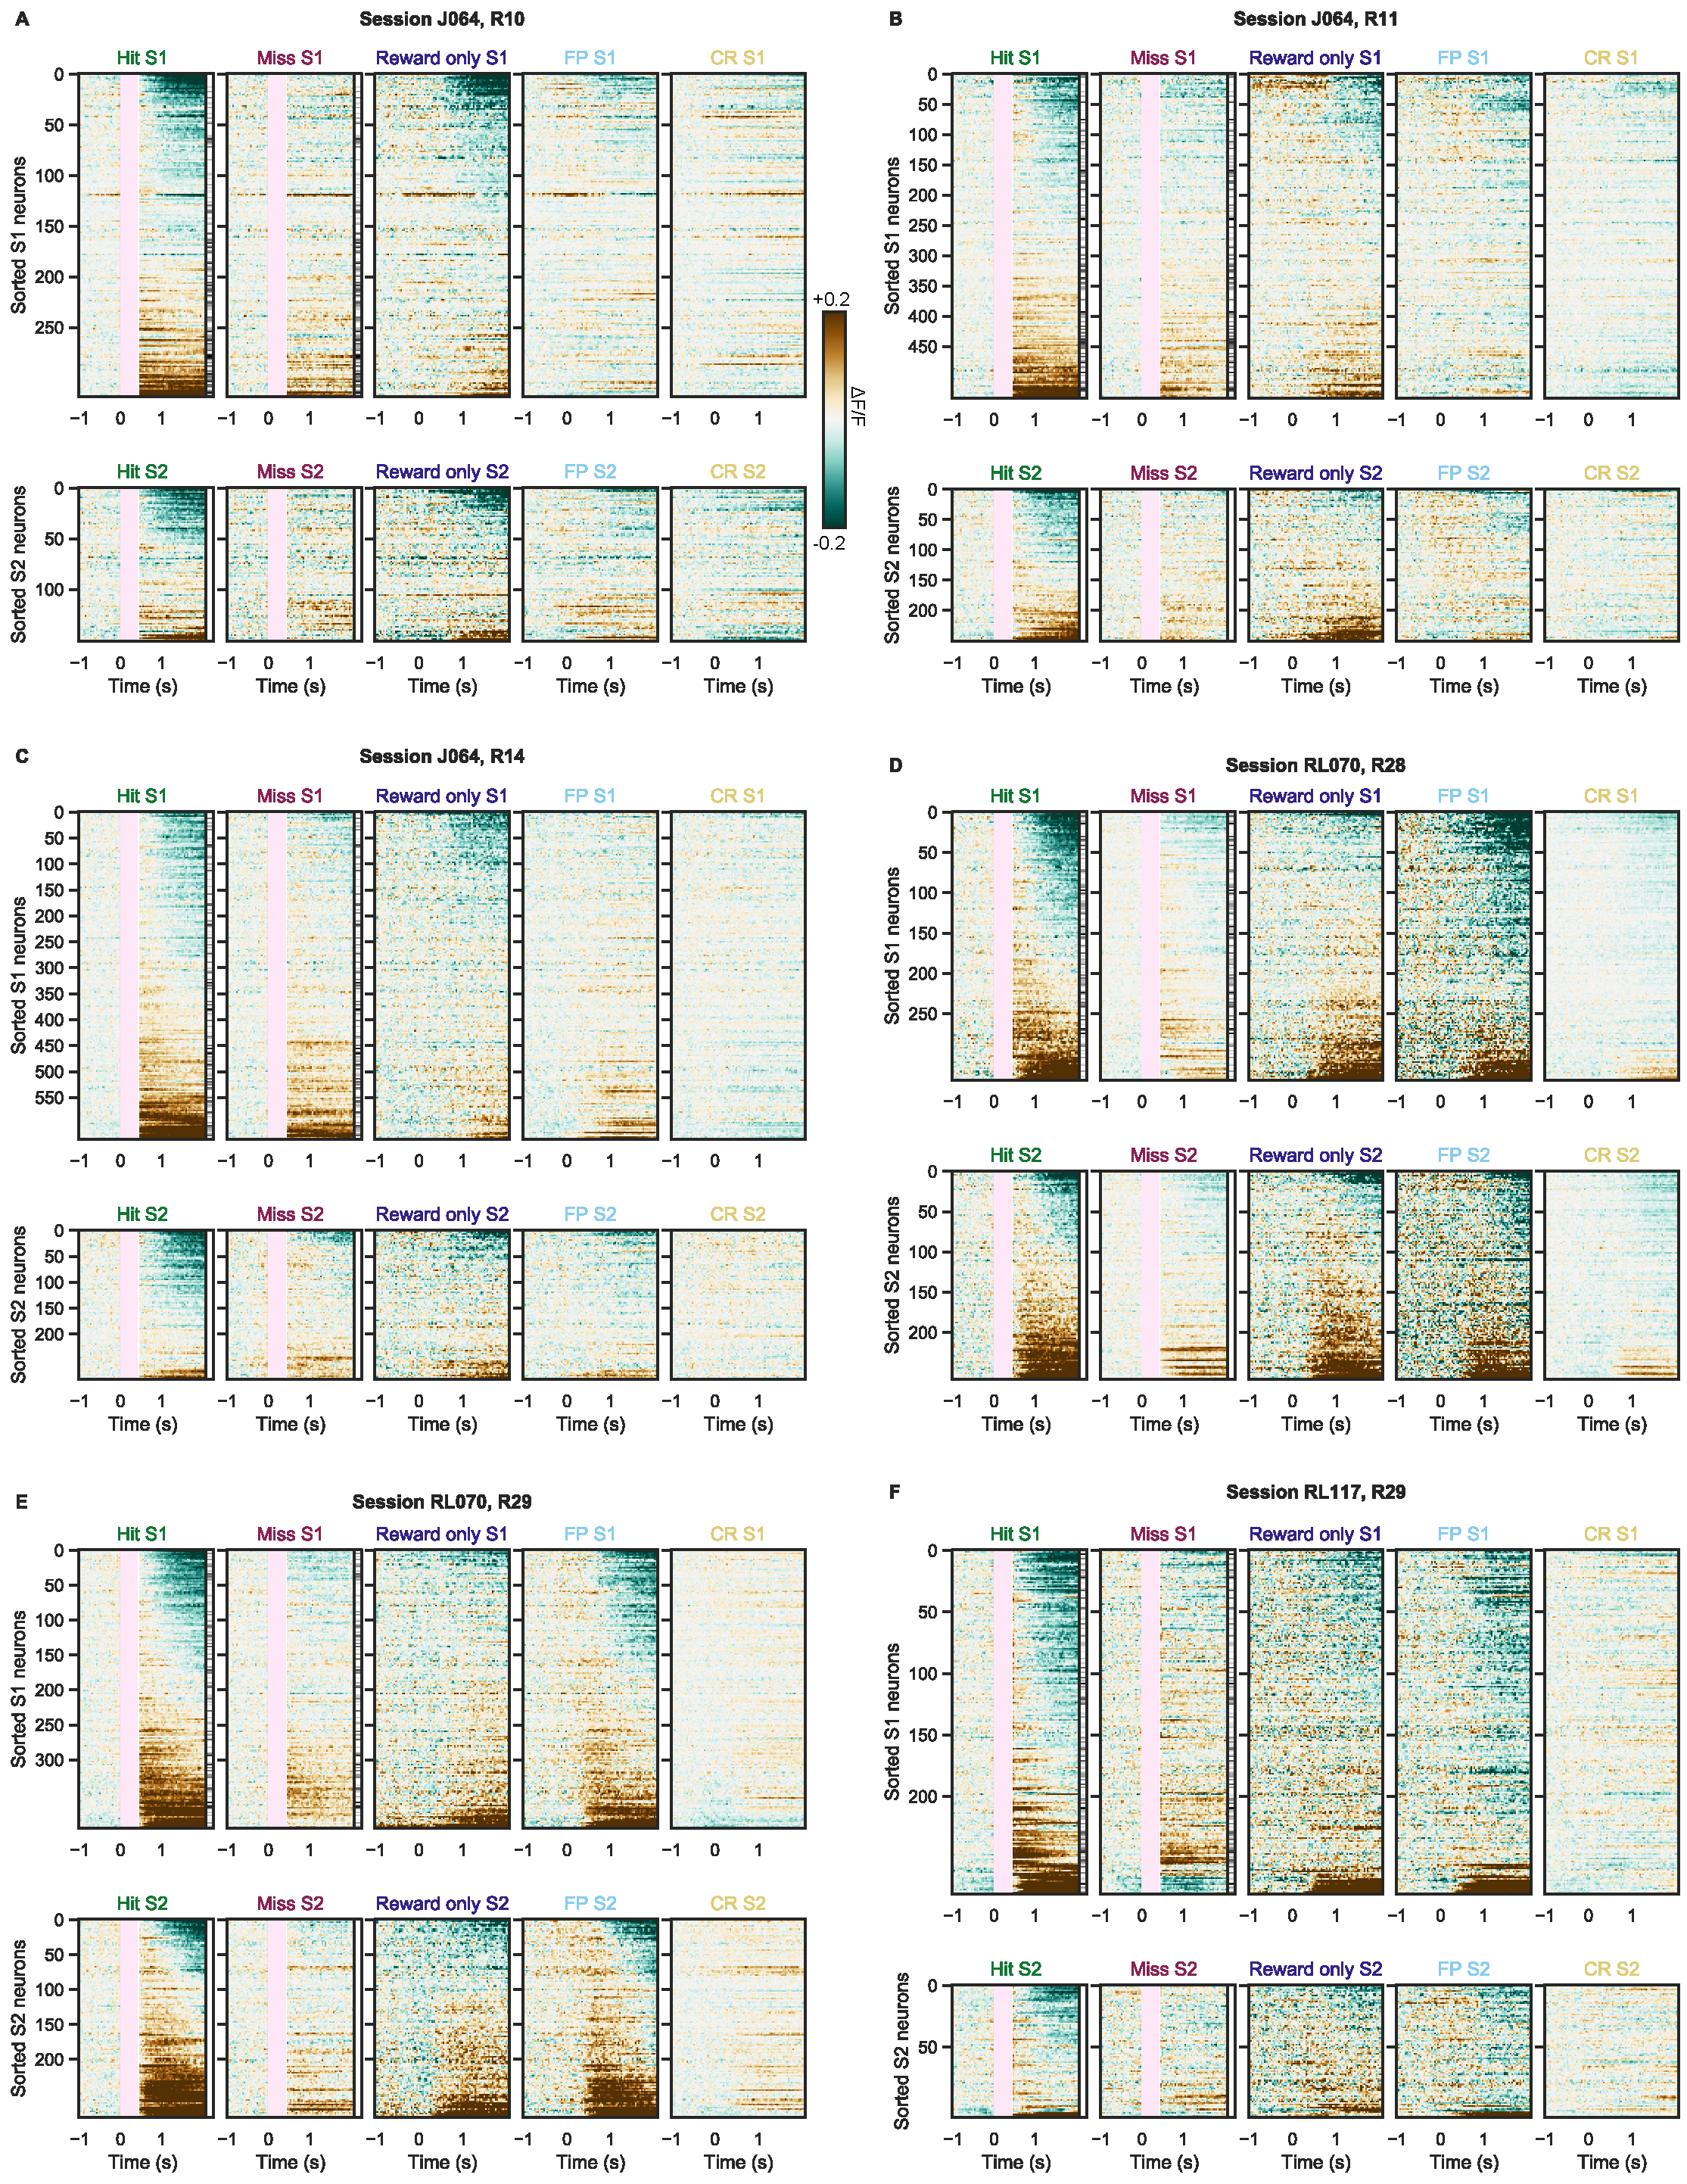
\includegraphics[scale=0.45]{figures/supplements/Supplementary_Figure2.pdf}
\caption[\textbf{Trial averaged raster plots for all sessions and trial types}]{\textbf{Trial averaged raster plots for all sessions and trial types}
\textbf{(A-F)} Raster plots showing the trial averaged response to trial types to photostimulation (pink vertical bar, hit/miss) and/or reward (hit/reward only) and/or licks (hit/reward only/false positive) of individual cells from 6 sessions. Data were baselined to the pre-stimulus mean on a cell-wise basis before averaging. Cells are sorted by the pairwise correlation between their trial averaged responses across all three trial types.
} 
\label{fig:supp2}
\end{figure}

\begin{figure}[h]
\hspace*{-0.6in}
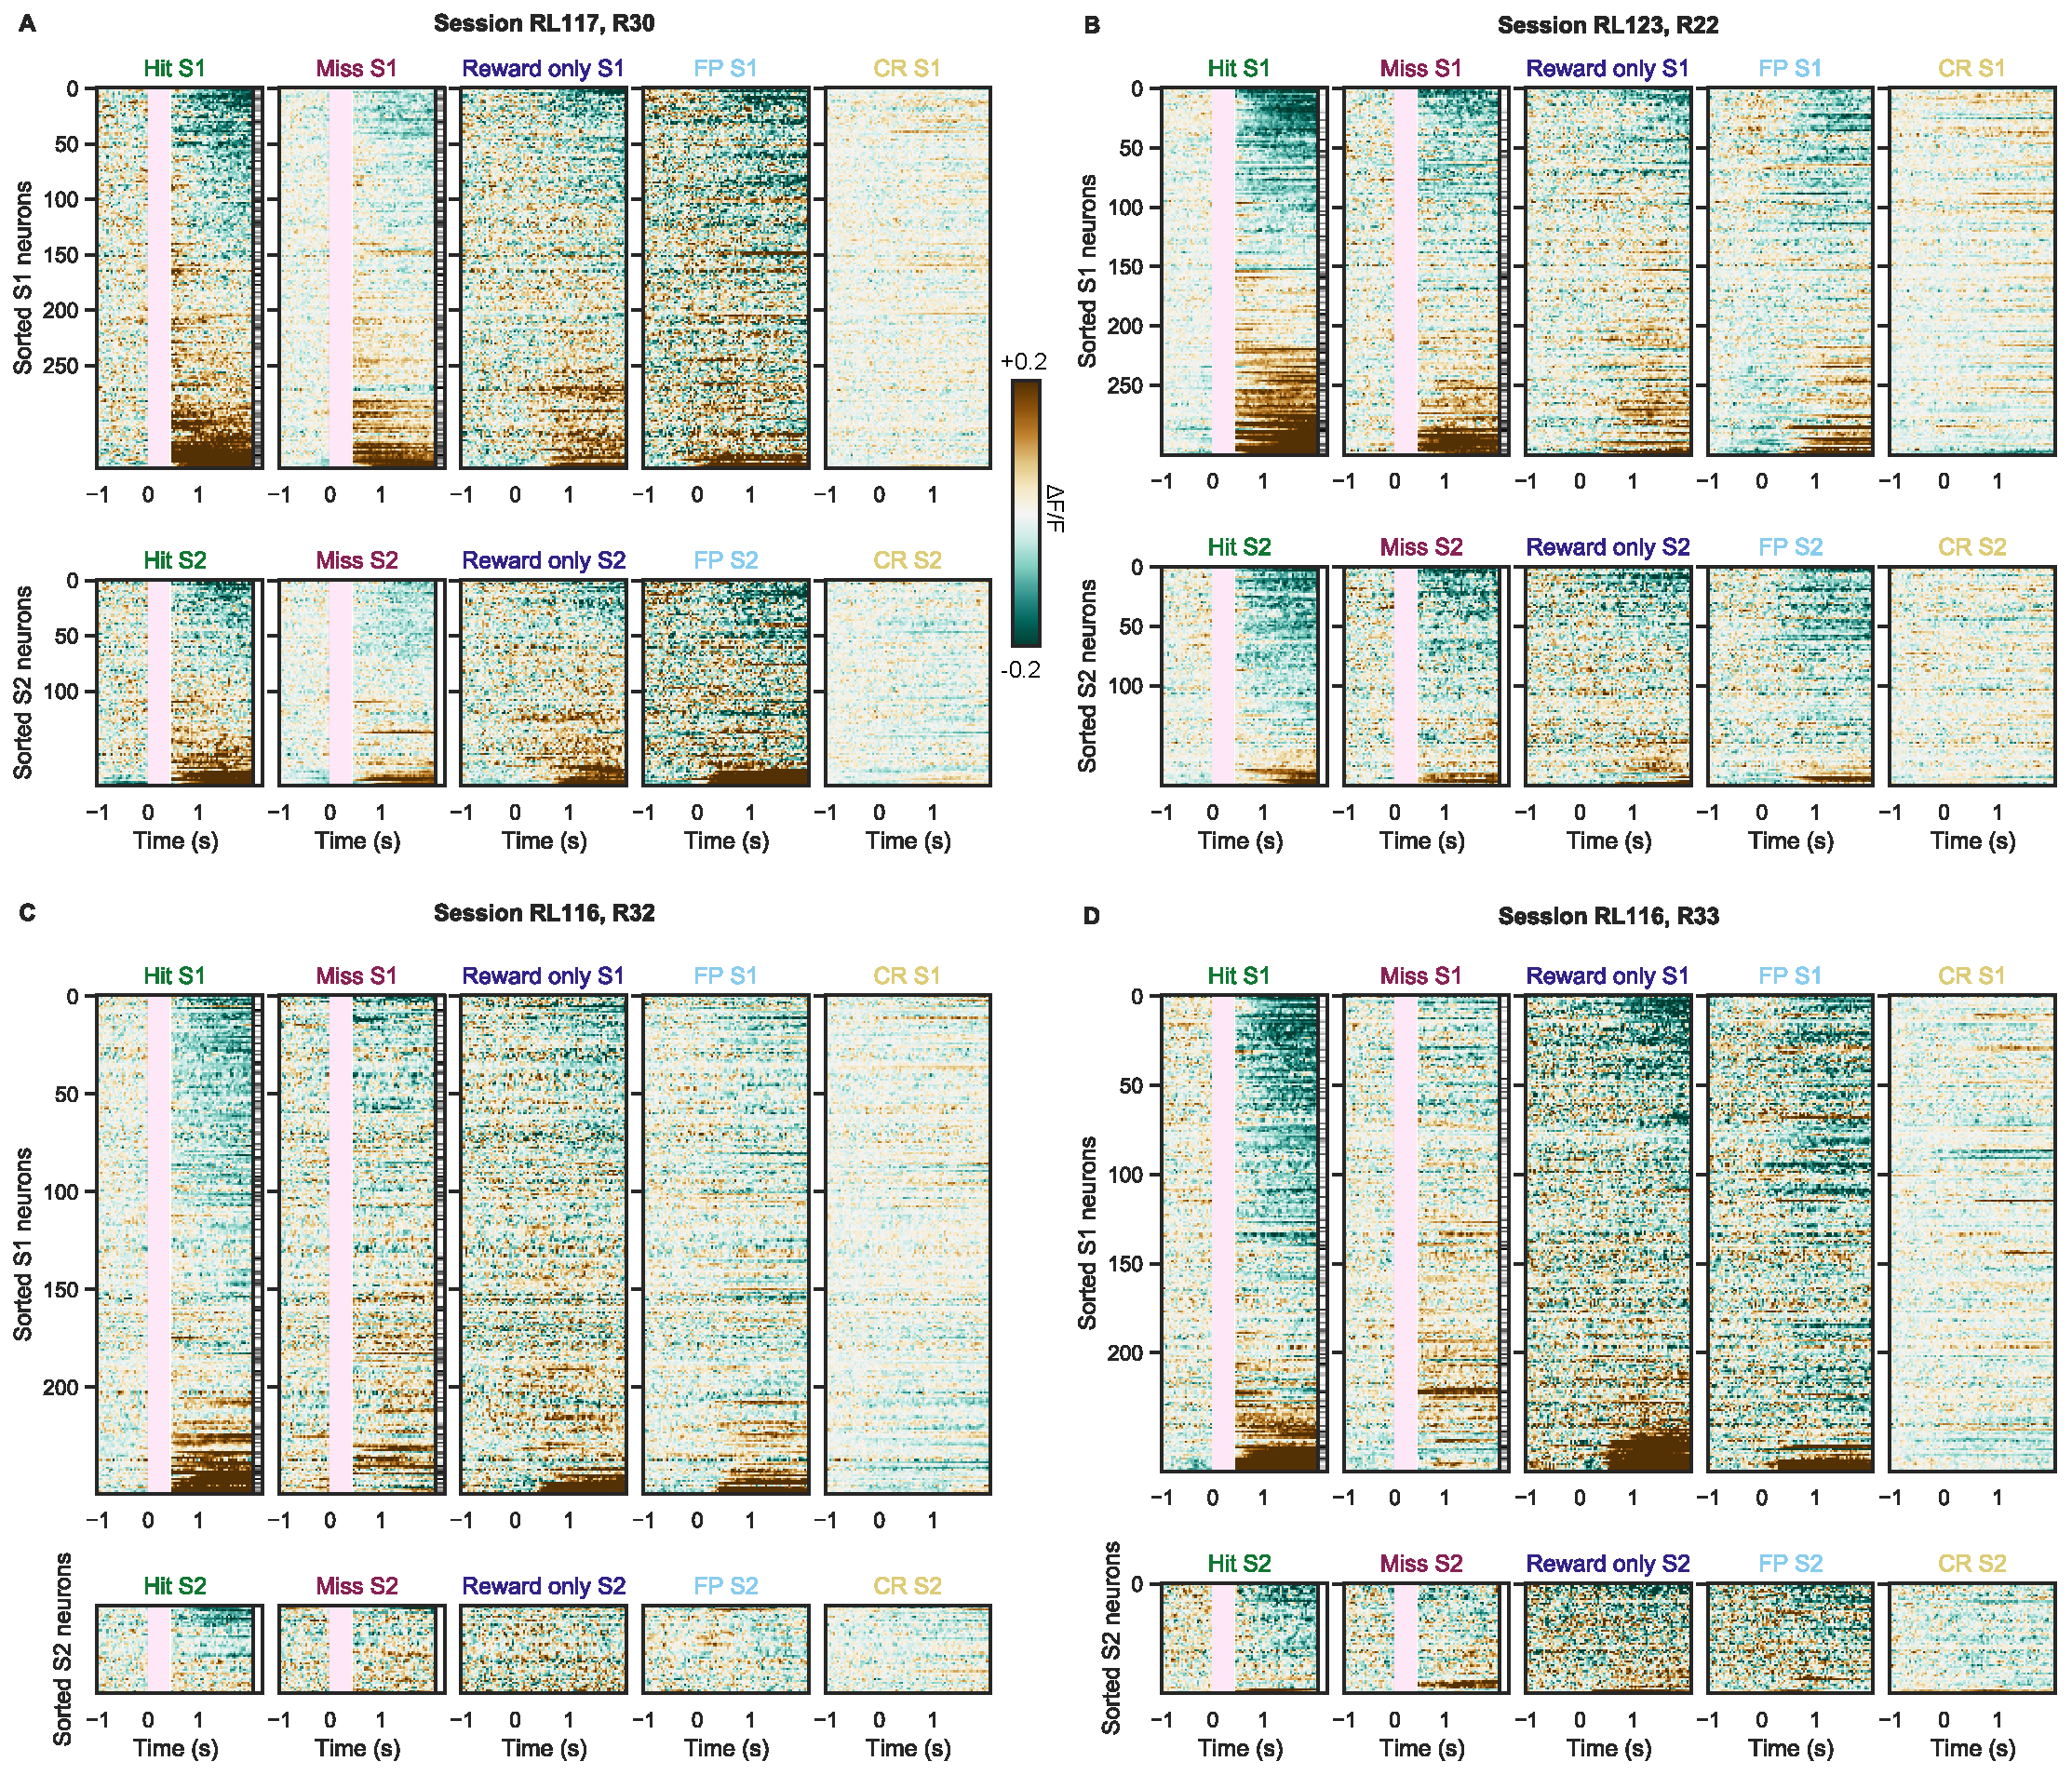
\includegraphics[scale=0.45]{figures/supplements/Supplementary_Figure3.pdf}
\caption[\textbf{Trial averaged raster plots for all sessions and trial types: continued}]{\textbf{Trial averaged raster plots for all sessions and trial types: continued}
\textbf{(A-D)} As above for the remaining 4 sessions
} 
\label{fig:supp3}
\end{figure}

\section{Perceived photostimulation elicit persistent activity in both S1 and S2 populations}

As shown in the previous section, individual cells display a diverse array of responses, and balanced mean average responses mask the magnitude and time course of propagated activity (Figure \ref{fig:basic-analysis}). To gain insight into these complex neural responses, we employed logistic regression classifiers on the network level and assessed propagation of stimulus-relevant activity and its relationship to behaviour. We trained classifiers to decode the trial type of individual trials using the activity of all cells in S1 or S2 on imaging data from single imaging frames. This allowed us to uncover the neural signatures of each trial type in both brain regions and quantify the temporal dynamics of this signature. First, we trained a model to classify hit trials from correct rejection trials, meaning the model should detect the neural signature of both the stimulus and the activity resulting in its perception. The classifier performed significantly above chance after stimulation and performance remained well above chance for several seconds both in S1 and S2 (two-sided Wilcoxon signed-rank test, p < 0.05, Bonferroni corrected) (Figure \ref{fig:fig3}A left, B left; Figure \ref{fig:supp4}A,B,G,H; Figure \ref{fig:supp5}A left, B left). Therefore, the neural activity underpinning perceived stimulation persisted both locally in S1 and downstream in S2 for several seconds. However, the classifier could be decoding the signatures of reward and the motor command required for licking, which are present on hit trials but not correct rejection trials. To address this, we tested the pre-trained classifier on reward only trials in which reward was delivered in the absence of photostimulation. In S1, performance on this trial type was either below or at chance level (p < 0.05, Bonferroni corrected); in S2, classifier performance on reward only trials remained at chance throughout the first 2.7 seconds of the trial (Figure \ref{fig:fig3}A left, B left; Figure \ref{fig:supp4}A,B,G,H; Figure \ref{fig:supp5}A left, B left) (p < 0.05, Bonferroni corrected). 


\begin{figure}[!h]
\hspace*{-0.2in}
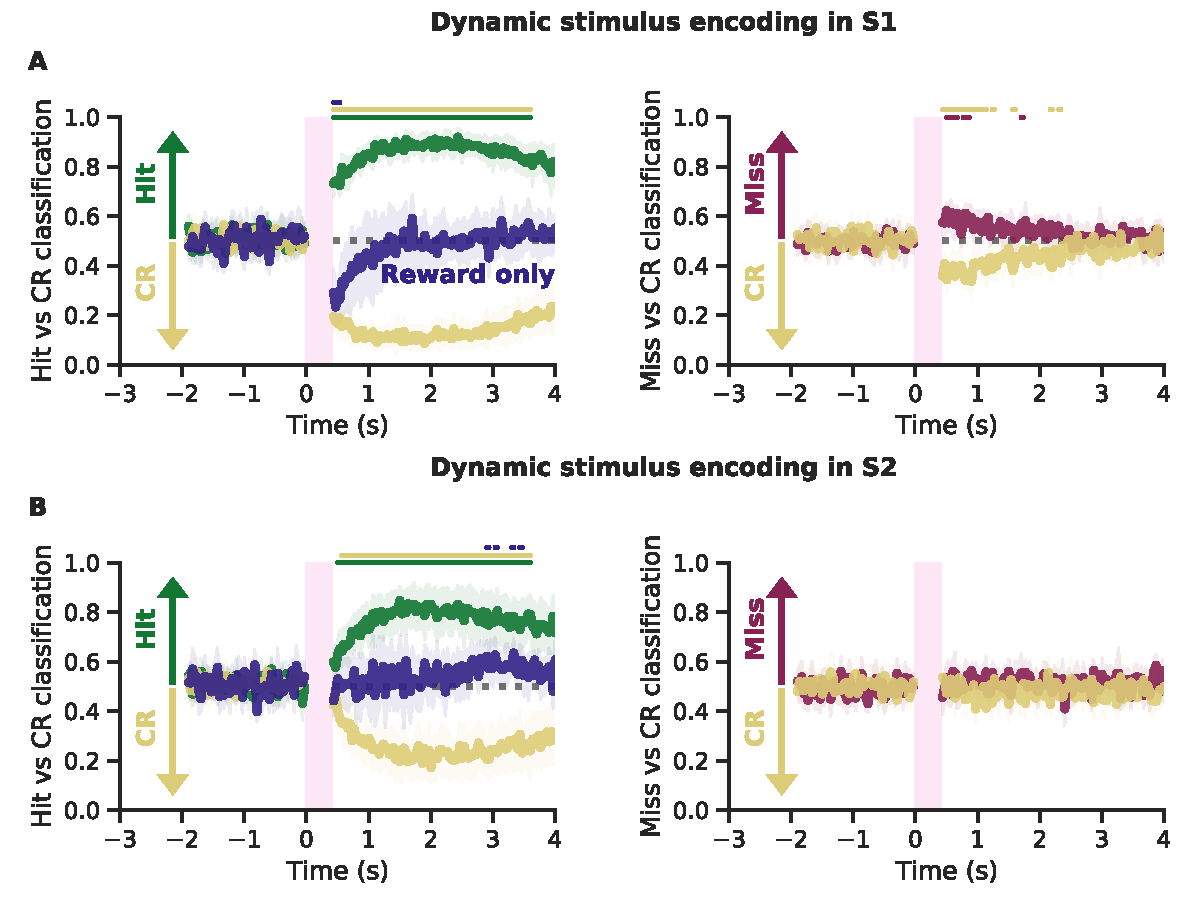
\includegraphics[scale=0.76]{figures/Figure3.pdf}
\caption[\textbf{Perceived photostimuli elicit persistent activity in both S1 and S2 populations.
}]{\textbf{Perceived photostimuli elicit persistent activity in both S1 and S2 populations} Dynamic decoding of trial type from neural activity in S1 using a logistic regression model. Models were trained on each frame individually, with activity from every cell in S1 or S2, and tested on held out data. Coloured bars above the traces show timepoints at which classifier performance was significantly different from chance (see methods).
\textbf{(A)} \textit{Left}: A model was trained on S1 activity to classify hit trials from correct rejection trials and then tested on hit trials (green), correct rejection trials (yellow) and reward only trials (blue). The model is able to classify hit trials from correct rejection trials for several seconds following photostimulation, implying that activity arising from perceived stimulation persists in S1. Reward only trials were not classified as hits, showing that the model was not just trained to decode the neural signature of reward on hit trials. \textit{Right}: A model was trained on S1 activity to classify miss trials from correct rejection trials and then tested on miss trials (red) and correct rejection trials (yellow). The model is able to distinguish the two trial types for only for ~1 second following stimulation. This implies that non-perceived stimuli do not generate persistent activity. \textbf{(B)} \textit{Left}: A model was trained on S2 activity to classify hit trials from correct rejection trials and then tested on hit trials (green), correct rejection trials (yellow) and reward only trials (blue). As above, the model is able to classify hit trials from correct rejection trials for several seconds following photostimulation, implying that activity arising from perceived stimulation in S1 is propagated to S2 and persists for several seconds. Reward only trials were not classified as hits, indicating that the model was not just detecting the neural signature of reward on hit trials. \textit{Right}: A model was trained on S2 activity to classify miss trials from correct rejection trials and then tested on miss trials (red) and correct rejection trials (yellow). The model was not able to classify miss from correct rejection trials at any timepoint, indicating that non-perceived stimuli were not robustly propagated from S1 to S2.
} 
\label{fig:fig3}
\end{figure}

\begin{figure}[!h]
\hspace*{-0.2in}
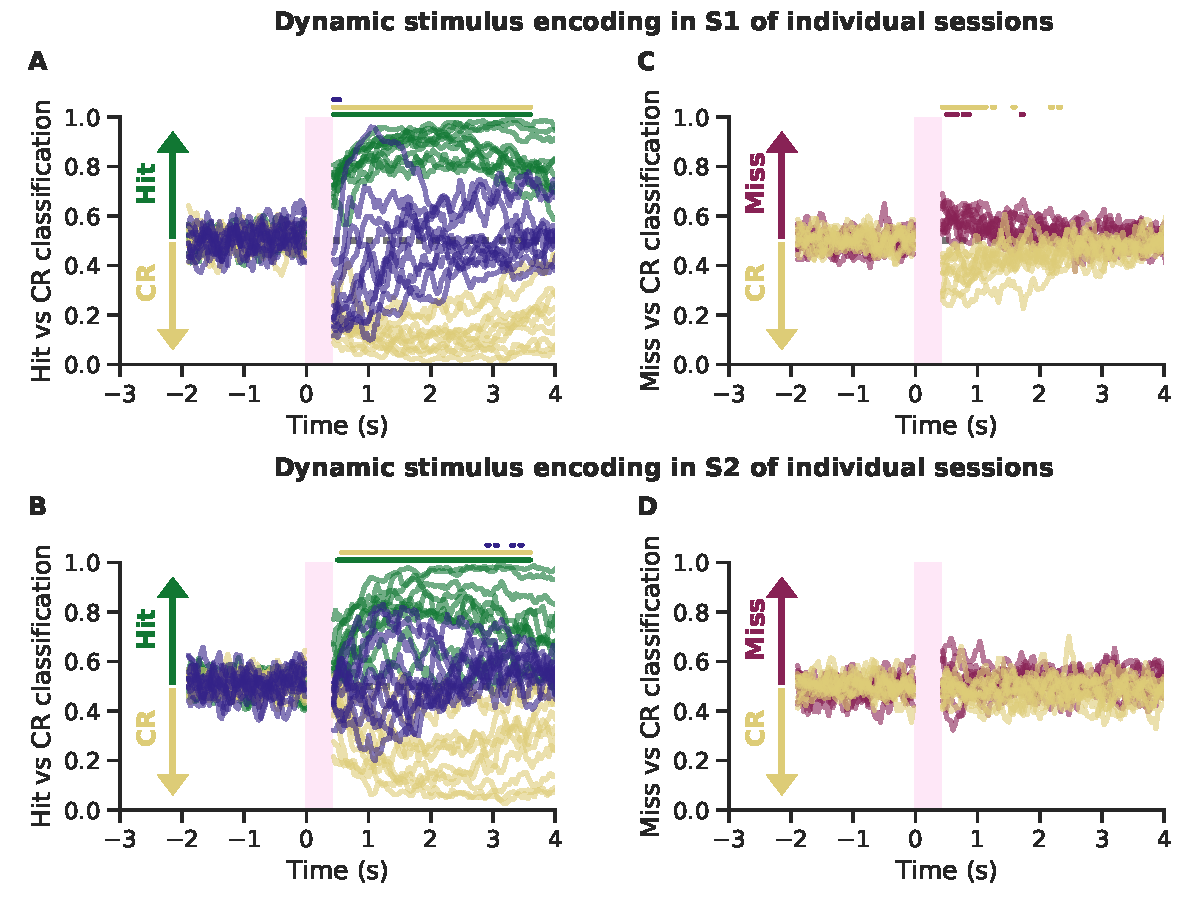
\includegraphics[scale=0.76]{figures/supplements/Supplementary_Figure5.pdf}
\caption[\textbf{Dynamic decoders of individual sessions}]{\textbf{Dynamic decoders of individual sessions} As figure \ref{fig:fig3}, but displaying classifier performance for each individual sessions. Individual sessions are shown as more transparent lines, with the session average as a fully opaque line.
} 
\label{fig:supp5}
\end{figure}

As reward signals in the brain are complex, and depend on whether the reward is expected or unexpected \cite{schultz_multiple_2000}, we confirmed that the reward signal on hit trials and reward only trials was comparable, thus ensuring that the hit vs correct rejection classifier was indeed classifying the neural signature of perceived stimulation and not just reward. This is critical as the water reward on hit trials was expected, but not expected on reward only trials. We addressed this by training a model to classify reward only trials from correct rejection trials, thus this classifier should detect only the neural signal from rewards (Figure \ref{fig:supp4}E,F). Testing this model on hit trials resulted in identical performance to the reward only condition both in S1 and S2 (no significant difference on 110/110 time points in S1 and 108/110 time points in S2). This means that a classifier trained specifically to detect rewards could not distinguish hit and reward only trials, meaning that the neural response to reward is comparable in both trial types and the classification of hit trials from correct rejection trials is indeed decoding the neural signature of perceived stimulation, both in S1 and S2.


\begin{figure}[h]
\vspace*{-3cm}
\thisfloatpagestyle{empty}
% \hspace*{-0.2in}
\vspace*{-0.2cm}
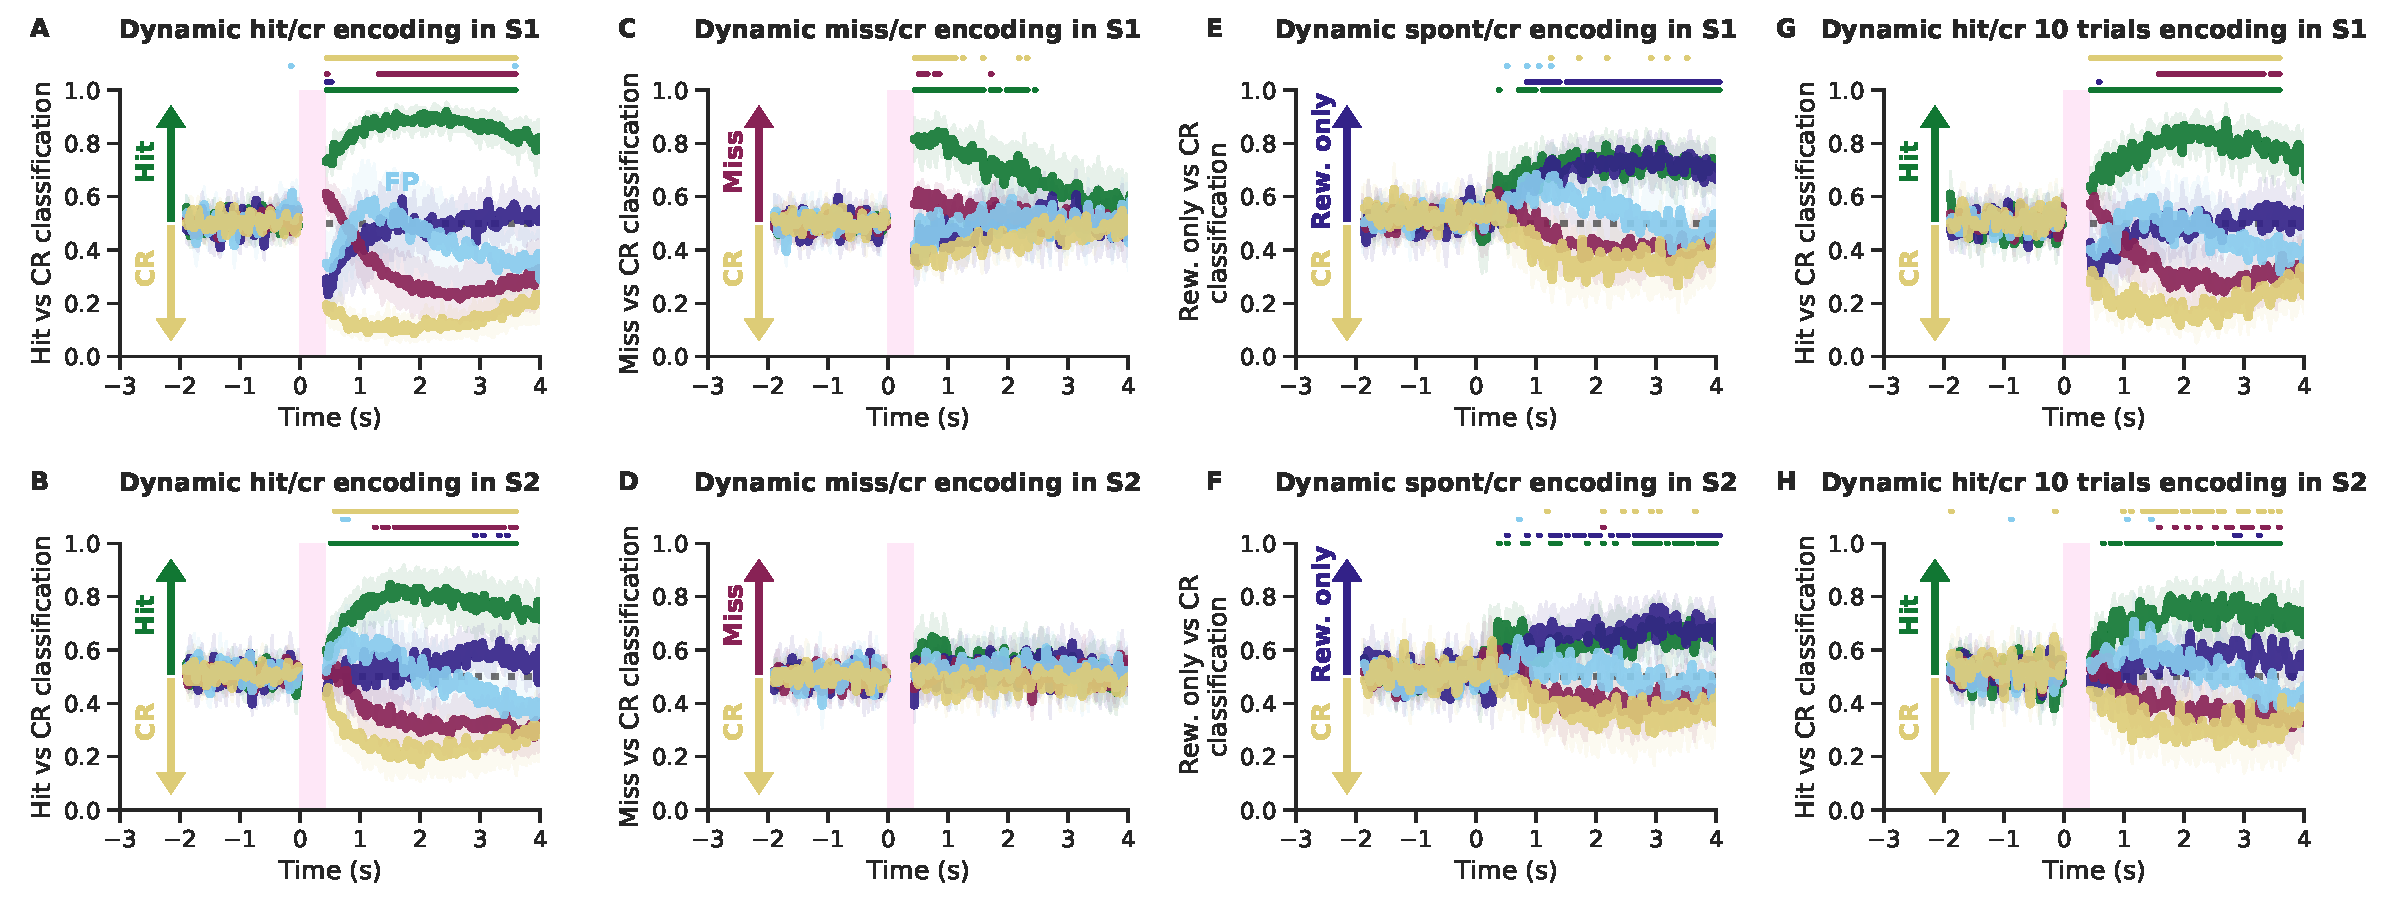
\includegraphics[scale=0.7]{figures/supplements/Supplementary_Figure4.pdf}
\caption[\textbf{Dynamic decoders of all trial types}]{\textbf{Dynamic decoders of all trial types} 

Dynamic decoding of trial type from neural activity in S1 using a logistic regression model. Models were trained on each frame individually, with activity from every cell in S1 or S2, and tested on held out data. Coloured bars above the traces show timepoints at which classifier performance was significantly different from chance (see methods). \textbf{(A)} A model was trained on S1 activity to classify hit trials from correct rejection trials and then tested on hit trials (green), correct rejection trials (yellow), reward only trials (dark blue), false positive trials (light blue) and miss trials (red). \textbf{(B)} As above, but trained on S2 activity. \textbf{(C)} A model was trained on S1 activity to classify miss trials from correct rejection trials and then tested on miss trials (red), correct rejection trials (yellow) reward only trials (dark blue), false positive trials (light blue) and hit trials (green). \textbf{(D)} As above, but trained on S2 activity. \textbf{(E)} A model was trained on S1 activity to classify reward only trials from correct rejection trials and then tested on reward only (dark blue), correct rejection trials (yellow), miss trials (red), false positive trials (light blue) and hit trials (green).\textbf{(F)} As above, but trained on S2 activity. \textbf{(G)} As \textbf{(A)} but the number of trials was restricted to 10 for each type, matching the total number of reward only trials recorded. \textbf{(H)} As \textbf{(B)} but the number of trials was restricted to 10 for each type, matching the total number of reward only trials recorded.
} 
\label{fig:supp4}
\end{figure}

Next we asked whether non-perceived neural activity was reliably propagated from S1 to S2 by training a model to classify miss and correct rejection trials (Figure \ref{fig:fig3}A right, B right; Figure \ref{fig:supp4}C,D; Figure \ref{fig:supp5}A right B right).

We found that in S1, this model decoded miss trials slightly above chance immediately following stimulation (p < 0.05, Bonferroni corrected), however performance rapidly decayed back to chance level after ~1 second. Conversely in S2, the model did not perform above chance at any point in time, indicating that stimulus information that is not perceived does not propagate to S2.

Taken together, these results show that only perceived stimulus representations are reliably propagated out of the local brain region in which they originate to a downstream brain area. Further, stimuli that are propagated and drive perception persist both locally and downstream for several seconds following the initial injection of activity.

\section{Pre-stimulus population in S1 predicts the upcoming trial outcome}

To address the conditions facilitating both the propagation of activity to S2 and the behavioural response to stimulus, we measured population activity in S1 immediately prior to stimulation (Figure \ref{fig:figure4}A) and asked whether any statistic of the pre-stimulus population activity could predict whether the stimulus would be perceived (i.e. whether the upcoming trial type would be a hit or a miss) (see methods). This allows us to assess how population activity is formatted pre-stimulus to gate whether the upcoming stimulation propagates and thus drives perception. One basic measure of population activity is the mean, measuring whether raised or suppressed activity across S1 prior to the stimulus arriving is predictive of an upcoming hit or miss trial. We find no evidence that this metric pre-stimulus is predictive of trial type (Figure \ref{fig:figure4}B left) (n.s.). Likewise, we find no evidence that the mean pairwise correlation between all pairs of neurons in S1 pre-stimulus increases or decreases the likelihood of stimulus detection (Figure \ref{fig:figure4}B center) (n.s.).


\begin{figure}[h!]
\vspace*{-1.5cm}
\thisfloatpagestyle{empty}
\hspace*{-0.4in}
% \vspace*{-0cm}
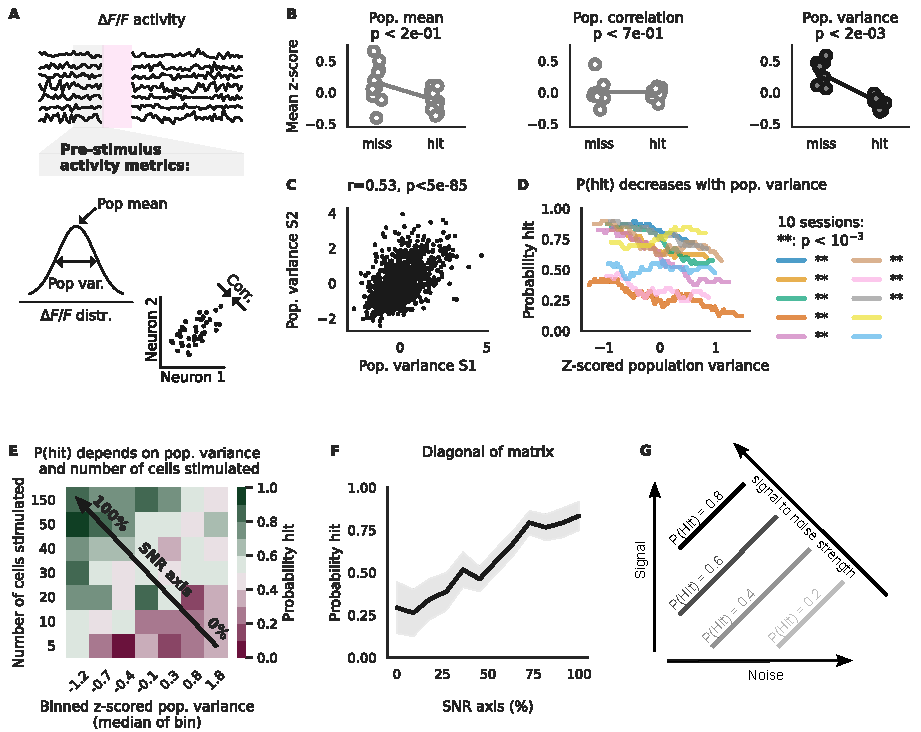
\includegraphics[scale=1.08]{figures/Figure4.pdf}
\caption[\textbf{Pre-stimulus population in S1 predicts the upcoming trial outcome}]{\textbf{Pre-stimulus population in S1 predicts the upcoming trial outcome} 

\textbf{(A)} Illustration of neural activity throughout a trial. Only the activity before the stimulus on a given trial is included in subsequent plots. We considered 3 metrics of pre-stimulus neural activity; the population mean, population variance and the average absolute correlation coefficient. \textbf{(B)} Comparison of population metrics of pre-stimulus S1 activity prior to hit trials and prior to miss trials. \textit{Left}: No evidence that mean population activity pre-stimulus predicts the upcoming trial outcome. \textit{Center}: No evidence that pre-stimulus pairwise Pearson correlation, averaged across all pairs of neurons, predicts upcoming trial outcome. \textit{Right}: Population variance is significantly higher before miss trials than before hit trials. Pre-stimulus population metrics in S1 were computed trial-wise and z-scored across trials within a session before being split into hit and miss trials and averaged across a session. P values tested for a difference in session-wise population metrics between hit and miss trials. \textbf{(C)} Population variance is significantly correlated between S1 and S2 on a single-trial level. \textbf{(D)} The probability of a hit trial as a function of pre-stimulus population variance in S1 on a single session level. Trials within a session were binned by their z-scored population variance and this was correlated to the probability of a hit trial within that bin. 8/10 sessions show a significant negative correlation between pre-stimulus population variance and the probability of a hit. \textbf{(E)} The interaction between pre-stimulus population variance in S1 and the number of cells photostimulated defines the probability of a hit trial. Trials within a session were binned by their z-scored population variance and by the number of cells photostimulated; the probability of a hit within each bin was plotted on a 2-dimensional axis. This was repeated for all sessions. Maximising the number of cells stimulated and minimising the pre-stimulus variance yielded the greatest probability of a hit trial. \textbf{(F)} Maximising the SNR of the stimulus resulted in the maximal probability of a hit trial. Data as in f, but projected onto the ‘SNR’ axis by averaging across all bins that project orthogonally onto each point on the axis. \textbf{(G)} Schematic outlining the intuition for the SNR axis. Increasing the number of cells stimulated on a given trial maximises the signal of that stimulus. Noise is inversely proportional to the population variance as there is more excitation and suppression from baseline in a population with high variance. The probability of hit is maximal when SNR is maximal as the stimulus is more likely to be detected above ongoing activity. 
} 
\label{fig:figure4}
\end{figure}

One metric that clearly predicts whether the upcoming stimulus will be propagated out of S1 to drive a hit is the population variance  (Figure \ref{fig:figure4}B right), defined as the variance of the distribution of activity across S1 neurons. The lower the variance of the activity distribution pre-stimulus, the more likely the upcoming trial will be a hit. Prior to a miss trial, the variance of activity across neurons is greater than prior to a hit trial (p < 0.002). See Figure \ref{fig:supp6} for the further quantification of significant activity metrics of both S1 and S2.  Additionally, population variance in S1 is correlated to population variance in S2, (Figure \ref{fig:figure4}C) (Pearson’s r = 0.53, p < 5x10\textsuperscript{-85}) demonstrating that this phenomenon is not just limited to the directly photostimulated brain region and therefore may be a metric of a more global brain state.


\begin{figure}[h!]
\vspace*{-1.5cm}
\thisfloatpagestyle{empty}
\hspace*{-0.6in}
% \vspace*{-0cm}
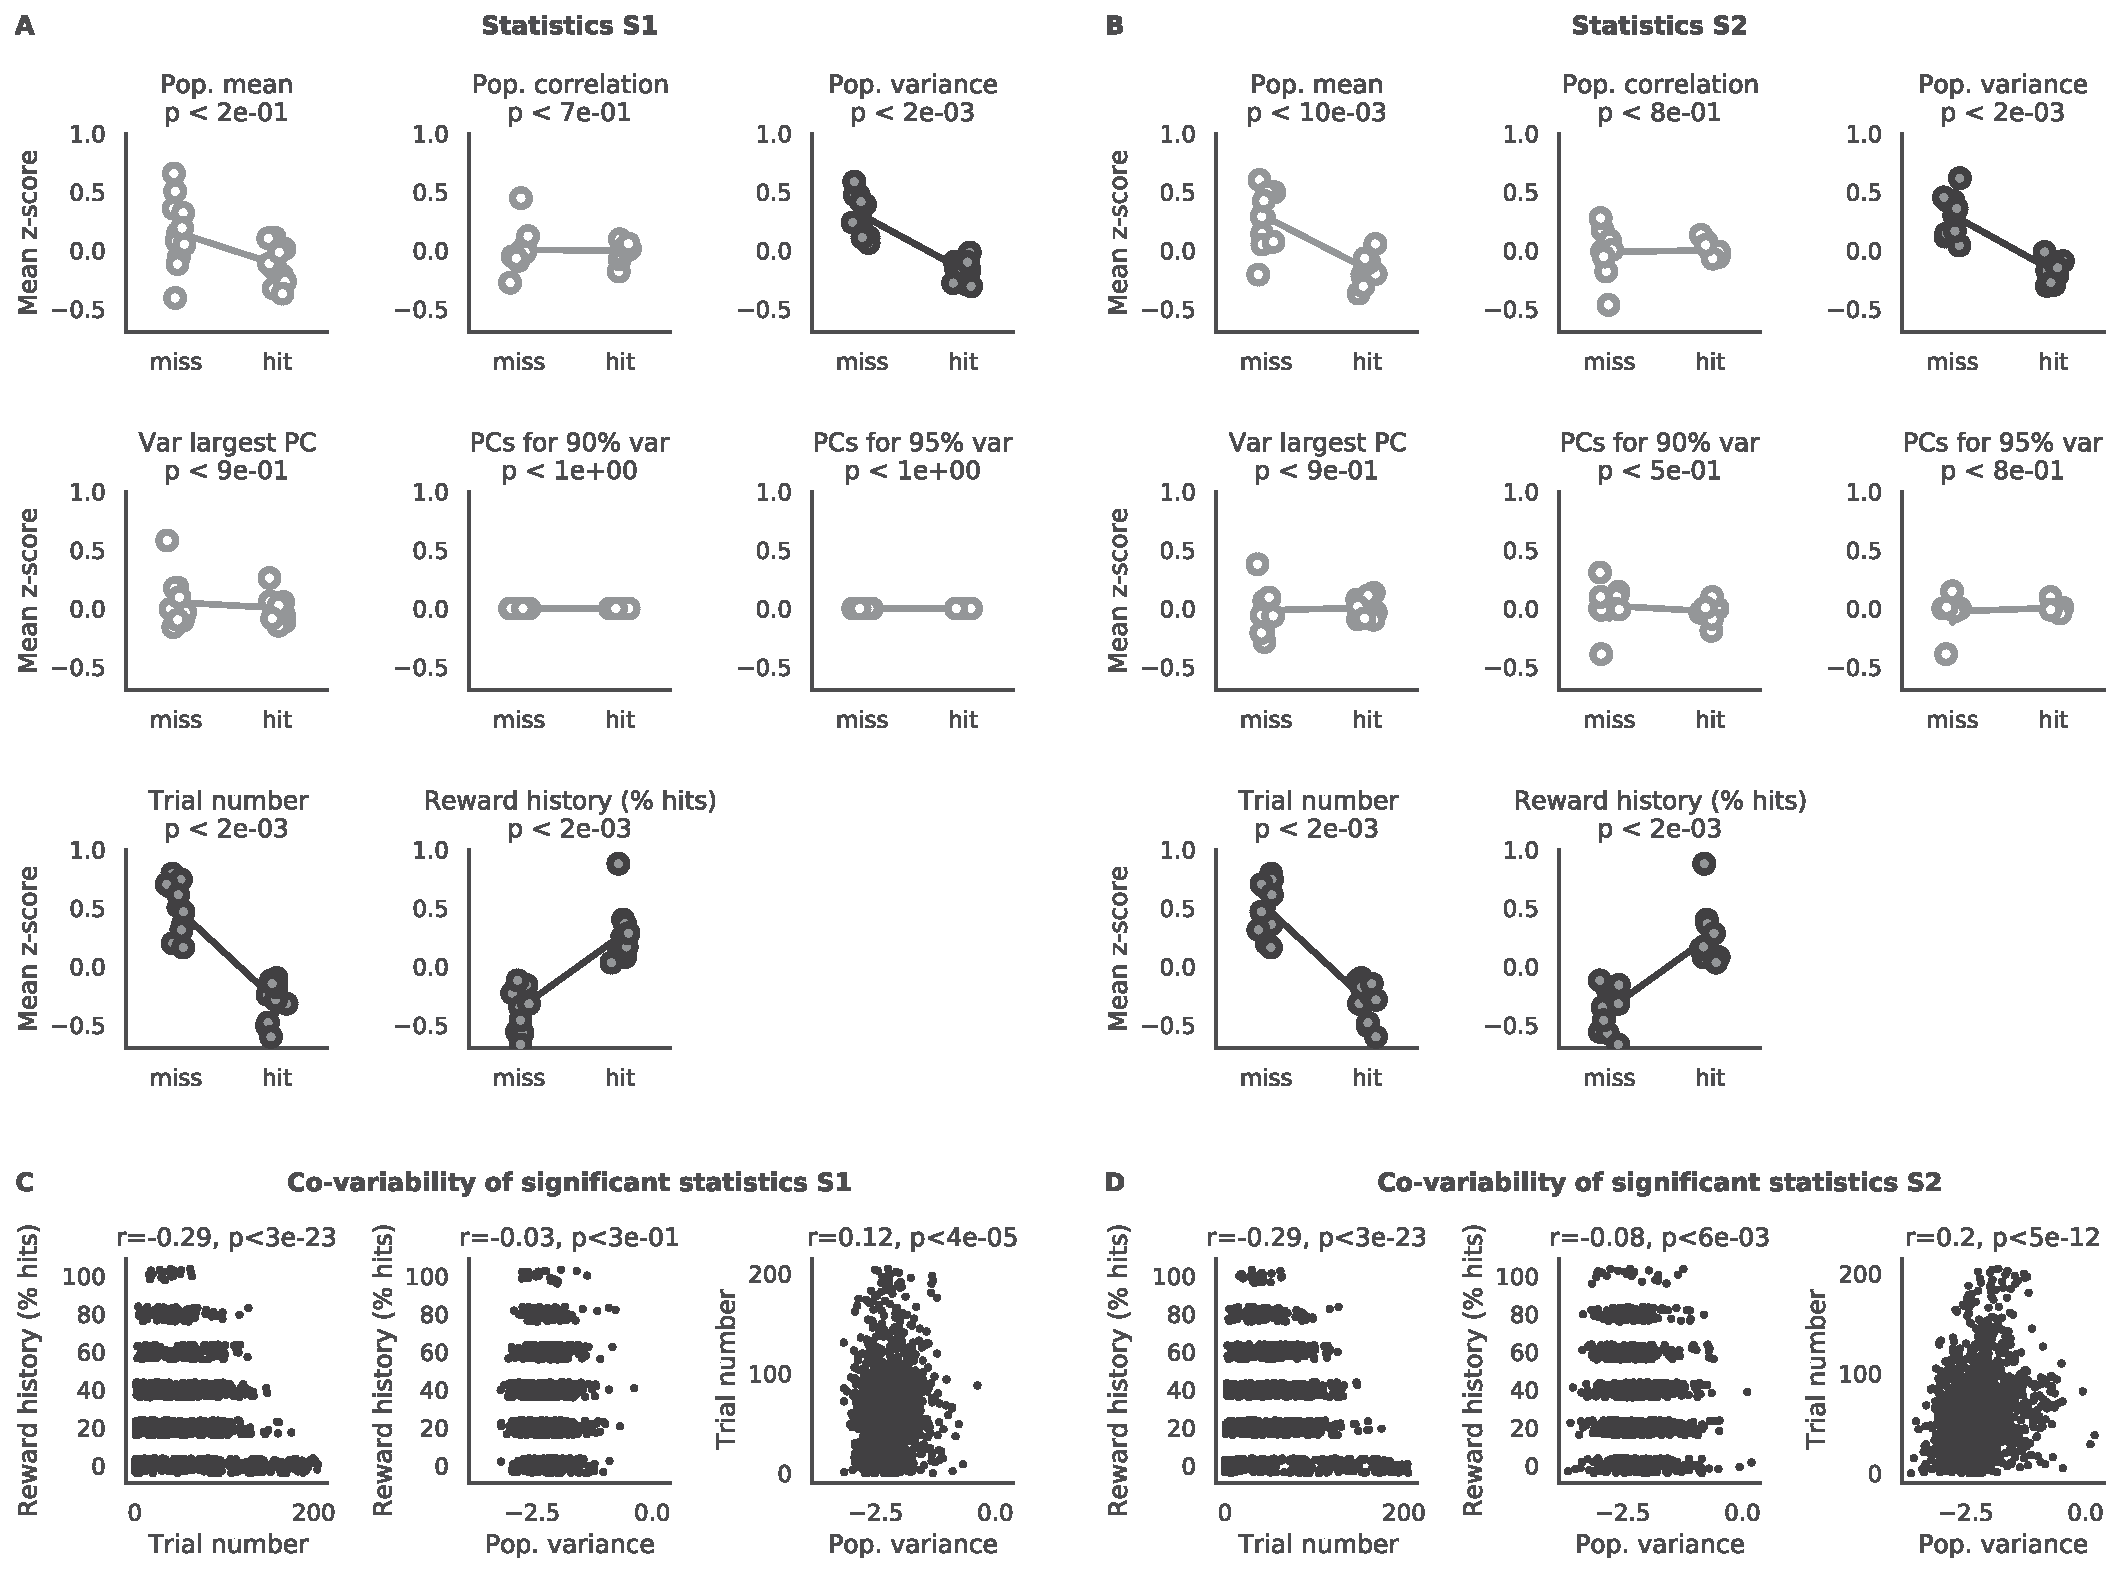
\includegraphics[scale=0.48]{figures/supplements/Supplementary_Figure6.pdf}
\caption[\textbf{Further population metrics of pre-stimulus activity
}]{\textbf{Further population metrics of pre-stimulus activity
} 
Comparison of population metrics of pre-stimulus in  S1 \textbf{(A)} and S2 \textbf{(B)} activity prior to hit trials and prior to miss trials. The top rows show the 3 metrics of Figure 4b. The middle rows show metrics computed using Principal Component Analysis (PCA) \cite{cunningham_dimensionality_2014}: the relative explained variance of the first Principal Components (PC), the number of PCs required for 90\% cumulative explained variance, and the number of PCs required for 95\% explained variance \cite{williamson_scaling_2016}. These are all metrics that indicate how well-structured, or low-dimensional, the covariance matrix is of the neural activity. These metrics are not significant which indicates that the change in population variance is not due a change in covariance structure. The bottom rows show two significant task variables; the trial number (an integer between 0 and the total number of trials in a session, indicating the number of trials previously undertaken by the animal in a given session) and the reward history (defined as \% hit trials in the 5 preceding stimulated trials). \textbf{(C,D)} The co-variability of the significant statistics of panels a and b was assessed using Pearson correlation. Reward history and trial number are strongly correlated, while population variance is significant but weakly correlated to trial number in S1 and both reward history and trial number in S2. 
} 
\label{fig:supp6}
\end{figure}


The relationship between population variance and behavioural performance was also evident on an individual session level, whereby population variance pre-stimulus in S1 is negatively correlated with the probability that the upcoming stimulus elicits a hit (Figure \ref{fig:figure4}D) (one-sided regression test p < 3x10\textsuperscript{-12} on 8/10 sessions, 1 session n.s., 1 session significantly increasing). This result, taken in conjunction with Figure \ref{fig:2-photon-behaviour}G, shows that we have identified two separate conditions that predict the probability that the animal will successfully perceive the stimulus: the strength of the stimulus (number of cells stimulated), and the variance of the population activity (Figure \ref{fig:figure4}B right, D). Next we asked if these two predictors work in tandem, where stimulus perception depends on both the strength of the stimulus and the ongoing state of the population.

We find a clear interaction in which the probability of a stimulus eliciting a hit can be expressed on a two-dimensional axis (Figure \ref{fig:figure4}E), where hit probability is highest when population variance is minimised and the number of cells stimulated is maximised. Stimulating just 5-10 neurons elicited a hit probability of greater than chance level (0.5) when pre-stimulus population variance was at its lowest level, whereas as population variance increased, more stimulated cells were required to reliably drive hits. This phenomenon can be well conceptualised in terms of a signal-to-noise ratio (SNR) framework, in which activity injected into cells through photostimulation forms the signal and the magnitude of background noise is measured as population variance. The higher the SNR, the more likely the animal is to detect the signal above ongoing noise and respond through a hit trial. Indeed, the probability of a hit is highly correlated with SNR when population variance and the number of cells stimulated are collapsed onto an SNR axis (Figure \ref{fig:figure4}F) (p< 2x10\textsuperscript{-10}, logistic regression two-sided t test). Taken together, these results show that the SNR of an incoming stimulus may be critical for its continued propagation out of the local brain region where it was initiated to downstream regions where it can drive behaviour (Figure \ref{fig:figure4}G).
\chapter{\label{discussion}Discussion}
Pioneering work in systems neuroscience has greatly evolved our understanding of how the sensory world is encoded in the cortex \cite{hubel_receptive_1962, okun_diverse_2015, stringer_high-dimensional_2019}. Additionally, critical to the brain’s ability to process stimuli is that activity is robustly propagated between functionally and anatomically distinct regions \cite{wernicke_aphasische_1874, felleman_distributed_1991, zylberberg_robust_2017}; however, much less is known about how neural systems coordinate to achieve this goal. While this question is often addressed in meso-scale studies of particularly the primate brain \cite{raichle_default_2001, van_den_heuvel_network_2013}, less is known about how the dynamics of neural activity are structured at the single-cell level to propagate activity between brain regions (but see \cite{reid_divergence_2001, semedo_cortical_2019, vugt_threshold_2018}). And as even spatially co-localised neurons can be functionally distinct \cite{runyan_response_2010, marmigere_specification_2007, kim_three_2015, velez-fort_stimulus_2014}, single-cell resolution recordings will be necessary to understand the journey of neural activity through the brain.

We have developed a preparation with key features crucial for studying activity propagation through the cortical hierarchy. First we record simultaneously from two hierarchically organised and densely interconnected brain regions (S1 and S2) with single cell resolution. Activity has previously been shown to readily propagate between these two regions \cite{pons_physiological_1987, alloway_homotypical_1985, kamatani_experience-dependent_2007, aronoff_long-range_2010} and communication between S1 and S2 has been shown to convey signals relating to active behaviour in addition to sensory stimuli \cite{kwon_sensory_2016, chen_behaviour-dependent_2013, chen_long-range_2016, yamashita_membrane_2013, yamashita_target-specific_2016}. 

Further, in our preparation, the neural activity driving behaviour is controlled experimentally. Behaviour driven through direct cortical stimulation provides a unique window into neural function as recorded neurons unambiguously generate behavioural actions. This greatly simplifies interpretation of recorded activity as, during sensory guided behaviour, neurons in the cortex are coupled to a vast array of external variables \cite{stringer_spontaneous_2019, musall_single-trial_2019}, as well as the internal brain state \cite{okun_diverse_2015, arieli_dynamics_1996}. In addition, neural activity passes through several synapses between the periphery and the earliest sensory cortical regions, adding a layer of computational complexity at each step \cite{mccormick_sensory_1994, sherman_thalamic_2005, king_superior_2004}. As a result, behaviour driven through direct cortical stimulation adds to our existing knowledge of cortical function, as the initiation of the neural activity underpinning behaviour can be directly recorded.

This idea has been implemented previously in mammals in a single brain region using both optical \cite{huber_sparse_2008, histed_cortical_2014, gill_precise_2020, dalgleish_how_2020} and electrical stimulation \cite{romo_somatosensory_1998, houweling_behavioural_2008, doron_spiking_2014, tanke_single-cell_2018, buchan_stimulation_2018}, demonstrating that animals can detect activation of small groups of neurons or even single cells; these studies generally employed repeated stimulation of the same neurons trial to trial. We expand upon previous literature by employing two-photon photostimulation and varying the number and identity of stimulated cells trial by trial. As such, we ensure that mice do not become sensitive to spikes in specific neurons and rather must tune into population events generated by co-activation of small groups of cells. This is critical as computation in the mammalian brain typically relies on populations of neurons acting in concert rather than the activity of single neurons \cite{averbeck_neural_2006}. Moreover, by performing stimulations spanning the perceptual threshold of the mouse, we were able to study population events in S1 that were detected and thus propagated to the downstream regions required to drive behaviour, such as those generating the motor command to initiate licking. We were then able to compare this to population events that were not reported by the animal. Finally, the behavioural response to two-photon activation of small groups of  S1 neurons has previously been thoroughly characterised \cite{dalgleish_how_2020}, and we demonstrate that this behavioural paradigm is robust and reproducible as our work finds that a similar number of activated cells is required to reach the inflection point on the psychometric curve pooled across animals. Our study is different to this previous work in that we vary the identity of stimulated cells trial by trial, rather than stimulating the same groups of neurons. As we find comparable behavioural results, this implies that populations of S1 neurons are able to generalise stimuli to elicit a behavioural report, regardless of the identity of the neurons stimulated.

\section{E/I balance}
We observe a diverse array of excitatory and inhibitory neural responses to two-photon photostimulation both locally in S1 and downstream in S2. While calcium imaging with GCaMP does not visualise inhibition explicitly, it has been shown that deviations of fluorescence traces below baseline is indicative of inhibition of tonically active neurons \cite{vanwalleghem_calcium_2021}. We find that on average, perceived stimuli (hit trials) are represented by a short period of excitation followed by a period of inhibition. This feature is expected from recordings made in S1 during whisker stimulation \cite{gabernet_somatosensory_2005, wilent_dynamics_2005}, however we show that it applies to activity arising directly from photostimulation in S1 and in activity in S2, propagated from S1.  Further we show that, in agreement with previous results \cite{dalgleish_how_2020}, S1 responds to excitatory two-photon photostimulation with a balancing inhibitory response. This is consistent with inhibition-stabilized networks (ISNs), formed from both strong excitatory and inhibitory recurrent connectivity. \textit{In silico}, strong excitatory connectivity enables amplification of input patterns \cite{murphy_balanced_2009}, persistent activity \cite{amit_model_1997}, and signal propagation between brain areas \cite{joglekar_inter-areal_2018} while inhibition tracks excitation to prevent unstable dynamics \cite{sanzeni_inhibition_2020}. We find evidence of amplification as stimulating 10s of neurons in S1 excites >5\% of recorded neurons, likely equating to hundreds or thousands of neurons total in the volume surrounding directly photostimulated cells. Next, perceived stimuli are decodable from both S1 and S2 for several seconds following photostimulation. As stimulation generally only transiently activates individual neurons, this is consistent with persistent activity resulting from recurrent connectivity \cite{daie_targeted_2021, seung_how_1996}. This is likely not only an artifact resulting from the long temporal dynamics of calcium imaging as our persistent activity lasts longer than would be expected from the temporal dynamics of GCaMP6s \cite{daie_targeted_2021, chen_ultrasensitive_2013}. Finally, we find that perceived stimuli are readily propagated from S1, and E/I balance extends to the downstream region S2 (although excitation and inhibition are less tightly coupled), consistent with data-constrained models of ISNs with long range connectivity \cite{joglekar_inter-areal_2018}. Taken together, we show that while populations of somatosensory cortex neurons exhibit a diverse range of responses to photostimulation of small groups of neurons, their activity is consistent with ISN models with recurrent connectivity. As perceived stimuli elicit both persistent and propagating activity, it is possible that recurrent connectivity consistent with ISN models, plays a role in this propagation.

\section{Stimulus generalisation}
We find that perceived stimuli (hit trials) are decodable from populations of neurons in S1 and S2, using a linear model. Our linear model classifies trial types in the held-out test set, on an individual trial level, based on the weighted sum of each neuron’s activity. However the weights are trained across the entire training set, formed from multiple trials. As a result, accurate decoding of the stimulus requires that individual neurons show a consistent increase or decrease in both training set and test set trials. Although we vary the identity of stimulated neurons trial by trial, hit trials are readily decodable from S1 and S2. This means that the neural response to perceived stimulation is comparable trial to trial in both brain regions, implying that the population generalises its representation of the stimulus. On miss trials, the presence of the stimulus is only decodable for a brief period in S1 immediately following stimulation, showing that non-perceived stimuli are not generalised across both brain regions. Stimulus generalisation is a well characterised phenomenon in psychology \cite{pavlov_conditioned_1927, pearce_model_1987}, biological circuits \cite{xu_neural_2013, henschke_reward_2020} and in artificial neural networks \cite{sietsma_creating_1991, jacot_neural_2018-1, summerfield_structure_2020}, and endows an agent with the ability to effectively interpret novel stimuli based on prior experience. This process has been shown to be enhanced if the stimulus is coupled to reward, matching our results \cite{henschke_reward_2020}. Hence we show that generalisation of neural activity is a feature of stimuli that are both perceived and propagated between brain regions. This generalisation is also observed in a downstream region from where the activity was initiated, implying that perceived neural activity may remain generalised throughout its journey through the cortex.

\section{Signal-to-noise ratio}
The signal-to-noise ratio (SNR) of a sensory neuron \cite{barlow_three_1969} or population of neurons \cite{zohary_correlated_1994} is often used to quantify the fidelity of the representation of a stimulus, whereby a higher SNR means that the sensory stimulus is more robustly represented as neural activity. Indeed, one of the functions of the highly recurrent circuitry in sensory cortex is thought to be the amplification of relevant activity arising from feedforward inputs, in order to enhance SNR \cite{douglas_recurrent_1995-1, ganguli_one-dimensional_2008}. Despite the well-characterised importance of high SNR in the local representation of sensory stimuli, less is known about how the SNR of a stimulus relates to its likelihood to propagate downstream. Here we replace the feedforward inputs employed \textit{in silico} with direct cortical activation and quantify noise as the population variance. We find that the probability a photostimulus was perceived, and was thus propagated downstream, is dictated by the SNR of the stimulus. The relationship between noise and signal propagation has been extensively studied in artificial neural networks \cite{vogels_signal_2005, diesmann_stable_1999, ozer_weak_2010, guo_signal_2011}. These studies show that a degree of ongoing noise is necessary for reliable propagation of activity packets between layers, however an excess of noise disrupts propagation \cite{guo_signal_2011}. These \textit{in silico} results are supported here as the cortex does not operate in a zero-noise regime \textit{in vivo} \cite{vreeswijk_chaotic_1998-1, faisal_noise_2008-1, anderson_contribution_2000, burns_spontaneous_1976, london_sensitivity_2010}, therefore we never observe a scenario where additional noise supports propagation. Taken together, we show that high signal-to-noise ratio activity is more reliably propagated between distinct regions of the mammalian cortex.

Although we find evidence that signal-to-noise ratio is a key neural feature facilitating activity propagation, we do not find evidence that inter-neuronal correlations are involved in this process. This appears to contrast with an elegant modelling study \cite{zylberberg_robust_2017} which showed that robust activity propagation between upstream and downstream cell layers was dependent on the covariance structure in the first layer. However this finding was made by varying the covariance matrix of the first layer on a trial by trial basis and examining the effect on the second layer. We are not able to control the covariance matrix of an entire cell layer \textit{in vivo}, hence further work is required to examine how the covariance structure of a population impacts its ability to propagate activity. 

In sum, this thesis examines for the first time how injecting activity into small groups of neurons in an upstream brain region impacts both behaviour and propagation of activity to a downstream region. Through this, we find indications that the somatosensory cortex operates as an ISN, that the connectivity structure of the ISN may assist in propagating activity and that both stimulus generalisation and signal-to-noise ratio are key neural features that may participate in ensuring robust stimulus propagation to coordinate brain regions and drive behaviour. 

\section{Futher work}
Further work with experimental manipulations of neural activity, such as two-photon photostimulation, is required to more closely examine how E/I balance, stimulus generalisation and signal-to-noise ratio impacts propagation of activity and its relationship to behaviour. Specifically, the causal link between these features of neural activity, behaviour and propagation could be further established using a closed-loop approach \cite{zhang_closed-loop_2018} whereby neural features such as noise are monitored online \cite{giovannucci_onacid_2017-1}. Photostimulation could then be delivered, for example, when the stimulated population is in a low-noise state and a high-noise state. Stimuli delivered in a low-noise state should elicit more robust propagation of activity and show an increased likelihood of driving a hit trial.  

It also follows from this work that feedback propagation of activity could be studied in the same framework. Most obviously, mice could be trained to report photostimulation of S2 neurons, while propagation of activity to S1 is monitored. Feedback of activity from higher to lower brain regions in the canonical pathway of sensory information flow plays a key role in many theories of cortical function \cite{rao_predictive_1999, lillicrap_backpropagation_2020}. Hence studying how feedback activity is propagated and the states employed by the brain to facilitate this could advance our understanding of cortical computation. Finally, it has been shown that mice can perceive optogenetic stimulation regardless of the brain region to which it is applied \cite{luis-islas_interoceptive_2021}. Hence the preparation described here could be applied to study any brain region, or the connections between them, and so further work could focus on whether propagating activity is shaped in the same way throughout the brain, or whether motor, frontal or subcortical regions employ a different strategy. Overall the experimental setup we describe here has great utility for assessing a wide range of brain regions, features of neural activity and theories of brain function.

\chapter{\label{ch:2-Materials and Methods}Materials and Methods} 

\minitoc

\section{Animal usage}

All experimental procedures involving animals were conducted in accordance with the UK animals in Scientific Procedures Act (1986).

Male and female C57/BL6 and Tg(tetO-GCaMP6s)2Niell mice were used for all experiments. Mice were between 4-12 weeks of age when surgery was performed.

\section{Surgical Procedures}
Animals were anaesthetised with isoflurane (5\% for induction, 1.5\% for maintenance) during all surgical procedures. A perioperative injection of 0.1 mg/kg buprenorphine (Vetergesic), 5 mg/kg meloxicam (Metacam) was administered. Mice were prepared for chronic imaging experiments through a single surgery. 2 mg/kg Bupivacaine (Marcaine) was applied to the scalp before it was sterilised with chlorhexidine gluconate and isopropyl alcohol (ChloraPrep) before being removed bilaterally. The skull was cleaned with a bone scraper (Fine Science Tools) to remove the periosteum. An aluminium head-plate with a 7 mm imaging well was bonded to the skull using dental cement (Super-Bond C\&B, Sun-Medical). A 3 mm circular craniotomy was drilled over the right somatosensory cortex, targeting the S1/S2 border (-1.9 mm posterior, +3.8 mm lateral), using a dental drill (NSK UK Ltd.). The skull within the craniotomy was soaked in saline before removal. Any blood was flushed with saline for >5 minutes, before a durotomy was performed. A single 1 μl viral injection was performed using a calibrated injection pipette bevelled to a sharp point. Injections were performed at a rate of 100 nl / minute at 300 μm below the pial surface and were controlled using a hydraulic micromanipulator (Narishige). 

 The majority of mice included in this work, and all those for which behavioural training was conducted, expressed the opsin C1V1-Kv2.1. To prepare these mice, pipettes were front loaded with either: 1:10 GCaMP6s (AAV1-Syn.GCaMP6s.WPRE.SV40) diluted in C1V1-Kv2.1 (AAV9-CamKIIa-C1V1(t/t)-mScarlet-KV2.1) if injecting into C57/BL6 mice or C1V1-Kv2.1 alone if injecting into transgenic mice. Some mice, used only for calibration of the two-photon photostimulation system, were injected with 1:10 GCaMP7s (AAV1-Syn-jGCaMP7s-WPRE), 1:7 ST-ChroME(AAV9-CAG-DIO-ST-ChroME-P2A-H2B-mRuby3) and 1:7 cre (AAV1-hSyn-Cre-WPRE-hGH), diluted in sterile PBS.

After injection, a double tiered cranial window composed of a 4 mm circular coverslip glued to a 3 mm circular coverslip was pressed into the craniotomy and sealed with cyanoacrylate (VetBond) and dental cement. Mice were recovered in a heated recovery chamber and kept under observation until behaving normally. Mice were subsequently monitored and their weight recorded for 7 days following surgery. Mice were allowed to recover for at least 21 days with ad libitum access to food and water before further procedures. This also allowed viral expression to ramp up before behavioural training was commenced.

\section{Two-photon imaging}
Two-photon imaging was performed using a resonant scanning microscope (2PPlus, Bruker Corporation) which raster scanned a femtosecond pulsed, dispersion-corrected laser beam (Vision-S, Coherent) across the sample at 30 Hz. A 16x/0.8-NA water immersion objective lens (Nikon) was used. GCaMP and mScarlet were imaged using a 920 nm and 765 nm beam respectively. Power on sample was controlled using a Pockels cell (Conoptics) and was kept at 50 mW for all experiments. A rectangular field of view (1024 x 514 pixels, 1397.4 x 701.4 μm), was used to image across two brain regions at 30 Hz. Imaging was controlled through PrairieView (Bruker Corporation).

\section{Widefield imaging}

Whisker stimulation during widefield calcium imaging was used to: target virus/tracer injections, determine the viability of a preparation for continued experimentation and find a suitable field of view for two-photon imaging encompassing S1 and S2 responses to a single whisker deflection. Using a camera, an LED and a dichroic/filter set, the whole cranial window was imaged using epifluorescence to measure calcium responses to whisker deflections. Each one of four whiskers (B1-B3 and C2; one at a time) was threaded into a capillary and deflected for 10 trials of 1 second each with 10 second inter-trial intervals. Each stimulation was 10 Hz and of ~300 um in amplitude at ~500 um from the base of the follicle. Responses to whisker stimulation were assessed using $\Delta$F/F stimulus triggered averages based on a baseline of 1 second pre-stimulus. Two areas of response moved stereotypically anterior-posterior and medial-lateral according to the row and column of the whiskers stimulated, confirming whisker responses were being assessed.

\section{Two-photon optogenetic stimulation}

Two-photon optogenetic stimulation was conducted using a pulsed fixed-wavelength fibre laser at either 1030 nm (Satsuma HP2, Amplitude Systèmes) or 1035 nm (Monaco, Coherent) at a repetition rate of 2 MHz. Multiple individual neurons were targeted for stimulation simultaneously by splitting the laser beam using a reflective spatial light modulator (SLM) (7.68 x 7.68 mm active area, 512 x 512 pixels, Boulder Nonlinear Systems). The active area of the SLM was overfilled and the polarisation optimised for maximal first order diffraction efficiency using a half-wave plate. The zero order diffraction beam was blocked using a well bored into an optical flat using a dental drill (NSK UK Ltd).

Phase masks were loaded onto the SLM using the blink SDK (Medowlark Optics). Phase masks were computed by applying the Gerschberg-Saxton algorithm \cite{gerchberg_practical_1972} to the xy coordinates of the target cell bodies. A weighted form of this algorithm was used to ensure uniform power distribution across all cells as the first order diffraction efficiency of the SLM is reduced with increasing distance from the zero order location. An image of the SLM was relayed onto a pair of galvanometer mirrors (Bruker Corporation) integrated into the two-photon imaging system. The galvanometer mirrors were programmed to generate spirals across cell somata by moving each beamlet simultaneously. Neurons were stimulated using 10 x 25 ms spirals of 15 \textmu m diameter and 6 mW power.

The affine transformation required to map coordinates from SLM space to imaging space was computed through a custom-modified version of open-source software written in MATLAB (github.com/llerussell/Naparm) using the two-photon image created by burning arbitrary patterns into a fluorescent plastic slide. Phase masks and galvanometer voltages required to perform photostimulation were generated using Naparm \cite{russell_influence_2019}. Voltages were applied to the galvanometers using PrairieView (Bruker Corporation). Custom written Python code was used to: select the cells for photostimulation, interface with Naparm to generate the files required to perform stimulation, interface with PrairieView to load voltage onto galvanometers and trigger photostimulation based on behavioural cues. A USB data acquisition card (National Instruments) running PACKIO \cite{watson_packio_2016}, was used as a master synchroniser to record the frame clock of the imaging, onset of photostimulation and a pulse to synchronise imaging and photostimulation with behaviour.

\section{Behavioural training}

Mice were water restricted and given access to \textasciitilde1 ml of water per day. Their weights were recorded and \textit{ad libitum} access to water or wet mash was provided if the animal's weight dropped below 80\% of the pre-restriction weight. For training, mice were head-fixed using their head-plate with their body supported in a 3d printed polylactic acid (PLA) tube. Mice became acclimatised to head-fixation and relaxed in the tube after the first 1-2 sessions. All behavioural training was controlled using the pyControl hardware and software \cite{akam_pycontrol_2021} based around the micropython microcontroller. The pyControl framework acted as the master clock for behaviour by writing the timing of behavioural input and output events to disk and triggering trials and stimuli based on behavioural events.

Mice reported photostimulation by licking a metallic lick spout placed \textasciitilde5 mm from the tongue using a micromanipulator arm (Noga Engineering). The spout was electrically connected to the pyControl lickometer circuit (Open-ephys), which both recorded licking events and drove a solenoid valve (Lee Products) to deliver a \textasciitilde2 \textmu l water reward.

The general structure of the task and individual trials was consistent at all stages of training. Each trial was separated by a fixed 5 second inter-trial-interval followed by a 4-6 second lick withhold period, where the length of the lick-withhold period was drawn randomly from a uniform distribution spanning these times. This prevented mice learning temporal structure in the task and eliminated the utility of a strategy based around random high frequency licking. If the mouse licked during the lick-withhold period, the trial was restarted and a new withhold length was drawn from the uniform distribution. 

Two trial types were delivered to the mice. During go trials, photostimulation was delivered and mice were rewarded if they licked to report perception of the stimulus. During catch trials, no photostimulation was delivered and mice were not rewarded if they licked the spout; no punishment was administered for licking on catch trials. 

The `response period' during which the mouse's licking response was recorded commenced immediately following the end of the lick-withhold period. This coincided with the onset of photostimulation in the case of go trials. The response period lasted for 1 second, and licks during this period alone were used to define the outcome of the trial. If the animal licked during the response period, this was scored as a `hit'; failure to lick on a go trial was scored as a `miss'. On catch trials, if the animal licked in the response period, the trial was scored as a `false positive'; trials where the animal did not lick in this period were scored as a `correct rejection'. A reward was delivered immediately after a correct lick on hit trials. This behaviour can thus be considered a detection task where catch trials are used to report the animal's baseline licking probability. Trial type was selected pseudorandomly ensuring no more than 3 consecutive trials of the same type. Mice were trained until they ignored 10 consecutive rewards or until 90 minutes had elapsed.

Behavioural performance was quantified using the d' metric \cite{brophy_alternatives_1986} which quantifies the difference in response probability between hit and catch trials while controlling for baseline response rate. This allows for comparison of performance of mice with conservative licking strategies, who are less likely to lick on both go and catch trials, with mice that are more likely to lick on both trial types.

d' is defined as:

\begin{equation}
d' = z(\text{hit rate}) - z(\text{false alarm rate})
\end{equation}

where: $z$ is the Z-transform function

The pyControl framework runs micropython, a lower level form of python compared to that available on a desktop computer and without any scientific packages. Hence, to perform calculation of d' online directly on the microcontroller, the Z-transforms of the hit and false alarm rates were calculated using a Pad\'e approximant:

\begin{equation} \label{eq:pade}
 R_{4,4} = \frac{\sqrt{2\pi}(P - \frac{1}{2}) - \frac{157}{231}\sqrt{2}\pi^{3/2}(P - \frac{1}{2})^{3}}{1-\frac{78}{77}\pi(P-\frac{1}{2})^{2} + \frac{241\pi^{2}}{2310}(P - \frac{1}{2})^{4}}
\end{equation}

where: $R_{4,4}$ is the 4th order Pad\'e approximation of the Z-transform and $P$ is the hit or miss rate.

\subsection{One-photon behavioural training}

Naive mice initially learned the association between photostimulation and reward through ‘one-photon’ widefield stimulation with a 595 nm LED (Cree). One-photon behavioural training was carried out in closed, light-proofed wooden boxes with the LED placed directly onto the cranial window using a micromanipulator arm (Noga). Current was supplied to the LED using pyControl and a custom designed analog driver board, allowing the power produced by the LED to be controlled programmatically. LED power was calibrated using a power meter (ThorLabs PM100D). A single trial's photostimulation consisted of 5 x 20 ms pulses over a period of 200 ms. LED stimulation was delivered on go trials only.

Initially, mice learned the association between optogenetic stimulation and reward through conditioning in which the stimulus was paired with reward regardless of the animal's response. Rewards that were delivered on miss trials are termed 'auto-rewards' and were delivered at the end of the response period. Mice rapidly learned to associate the optogenetic stimulus with reward and began licking before the auto-reward within 1-2 sessions. Mice were transitioned out of the auto-reward phase and into active training when they scored three consecutive hit trials. During active training, mice were not auto-rewarded aside from for a single trial if they registered 4 consecutive misses; this functioned to motivate poorly performing mice during a session.

During the initial training phase and the first stage requiring active responses,  LED power of 10 mW was used, with mice transitioned to progressively weaker LED powers once their performance was sufficiently high. Online performance was computed using running d', computed across a window of 10 trials. Once animals had reached a running d' of 2, the LED power was reduced in a stepwise fashion until the lowest power (0.1 mw) was reached. Once animals had exceeded criterion at this power, they were considered to have completed the one-photon training paradigm.

\subsection{Two-photon behavioural training}

After learning the one-photon stimulation task, mice were transitioned to the two-photon version of the task, whereby mice responded to two-photon photostimulation targeted to S1 only. Initially mice were trained on a task in which ~150 S1 neurons were photostimulated on every go trial in groups of 50, with an inter-group-interval of 5 ms.  Once mice registered a d' > 1.5 across an entire session, they were transitioned to the main version of the task. This task consisted of three trial types selected pseudorandomly, with equal probability and with no more than three consecutive trials of the same type. On 1/3 of trials, 150 cells were stimulated in groups of three, on 1/3 of trials, cells were stimulated in a single group, with the number of targets stimulated drawn randomly from the set \{5,10,20,30,40,50\} with equal probability and with replacement, the final 1/3 of trials were catch trials in which no photostimulation was performed. 

Before each session, photoresponsive cells were identified by performing two-photon photostimulation spanning opsin-expressing areas of S1. This generated the coordinates of ~150 S1 neurons known to be responsive to stimulation. The subset of neurons to be stimulated was selected randomly before each trial; cells in each simultaneously stimulated subset were no more than 350 μm apart. 

Prior to active behaviour, 10 minutes of spontaneous imaging was performed without any photostimulation being delivered. During this time period 10 rewards were delivered with an inter-reward-interval of 10 seconds; this allowed us to assess the ‘reward only’ neural response in somatosensory cortex. Active behaviour followed spontaneous imaging, during which the mouse was rewarded only if it responded to a go trial. Neural activity was imaged throughout active behaviour but was stopped every ~15 minutes to ensure the objective lens was completely immersed in water and to monitor animal welfare. The field of view was manually corrected for drift throughout the session by moving the objective to realign the field of view to a marker cell.

White noise was played to the animal throughout the session to mask auditory cues signifying the onset of stimulation and galvanometer mirrors were moved in an identical fashion on both go and catch trials. This ensured that the auditory cues generated were matched on both go and catch trials, and ensured that mice were responding to optical activation of S1 alone. Behavioural events were recorded through pyControl and photostimulation was controlled by custom written routines in Python and C.


\section{Imaging Data analysis}

Online analysis carried out during an experiment was conducted using STAMovieMaker (github.com/llerussell/STAMovieMaker). These stimulus triggered average (STA) images displayed visually the change in activity of each pixel in the field of view post-stimulus relative to pre-stimulus, thus the pixel intensity of the image was proportional to the increase in activity driven by photostimulation. STA images were trial averaged in a group-wise fashion and colored, such that pixels of a given color represent the average activity driven by repeated photostimulation of a given group of neurons. These images were used to manually define the coordinates of cells in S1 responsive to optical stimulation.

All further analysis was conducted offline. Calcium imaging movies were processed using Suite2p \cite{pachitariu_suite2p_2016} and regions of interest (ROIs) corresponding to putative cell somata were manually selected. Suite2p also extracts a signal arising from the neuropil surrounding a cell body. To remove contamination of the signal arising from individual soma by the surrounding neuropil, we subtracted the neuropil signal from each cell body at each timepoint (t) according to the equation:

\begin{equation} \label{eq:neuropil_sub}
F(t) = F_{soma}(t) - F_{neuropil}(t) \times 0.7
\end{equation}

where: \newline
$F$ = neuropil subtracted fluorescence \newline
$F_{soma}$ = fluorescence from the cell's soma \newline
$F_{neuropil}$ = fluorescence from the cell's surrounding neuropil \newline
0.7 = neuropil coefficient \cite{chen_ultrasensitive_2013} \newline

To ensure that cells with a bright baseline did not dominate the analysis, we computed $\Delta F/F$ for each cell using the equation:

\begin{equation} \label{eq:dff}
\Delta F/F = (F  - \Bar{F}) / \Bar{F}
\end{equation}

where: \newline
$\Bar{F}$ = The mean of $F$ across time through the entire session

Cells with very high $\Delta F/F$ values ($max(\Delta F / F) > 10 $) were discarded from further analysis.

Imaging data was split into individual trials, defined as 2 seconds preceding and 8 seconds proceeding the onset of a trial. Frames occuring while the photostimulation laser was on were excluded due to artifactual crosstalk in the imaging channel. Trial onset was defined either as the onset of photostimulation in the case of go trials, the onset of galvo spiralling in the case of catch trials or the delivery of reward in the case of reward only trials. 

Neurons were defined as ‘targeted’ on an individual trial if any part of their cell body was located within 15 μm of the centre of the photostimulus beamlet. Neurons were categorised as responsive or unresponsive to stimulus or reward in a trial-wise manner. For each trial, the distribution of $\Delta F/F$ values 500 ms pre-stimulus were compared to 500 ms post-stimulus for each cell. A cell was deemed as responsive to a stimulus on an individual trial if it passed a significance threshold of p = 0.05, using a two-sided Wilcoxon signed-rank test, following false discovery rate (FDR) correction. The alpha of the FDR correction (0.015) was set empirically as the value which yielded ~5\% of cells responding on correct rejection trials, where there was no stimulation or licking response. Following significance testing, cells were split into positive and negative responders based on whether the mean $\Delta F/F$ value post-stimulus was greater or less than the mean $\Delta F/F$ value pre-stimulus respectively.

\section{Pre-stimulus population metrics}

All pre-stimulus population metrics were computed across a 500 ms period immediately prior to photostimulation. All metrics were calculated on a trial-wise basis. The natural logarithm was taken of metrics that were fit better by a log-normal distribution as opposed to a normal distribution as assessed by Kullback-Leibler divergence. 

Mean population activity was computed by first averaging $\Delta F/F$ activity across all pre-stimulus frames for each neuron to yield a vector containing a scalar value for each neuron defining its pre-stimulus activity. Next firing rates were averaged across all neurons to give a single scalar value for each trial, defining the average population activity. 

Population variance was computed in a similar fashion, first by averaging across all pre-stimulus frames for each neuron. However rather than taking the mean of the activity vector as above, the variance of the vector was used to generate a single scalar value for each trial.

Mean pairwise correlation was computed by calculating the cross-correlation matrix for all pairs of neurons, whereby element i,j in this matrix was the Pearson correlation between neuron i and neuron j across all pre-stimulus frames. A single scalar value was generated for each trial by taking the absolute value of each element in the matrix, then computing the mean across all off-diagonal elements of this matrix.


\section{Normalisation and sorting of post-stimulus neural activity}

Post-stimulus neural activity was baselined relative to pre-stimulus activity in order to assess the relative change in activity after the photostimulation period, and to compare this change across cells and trials. On each trial, for each individual cell, the average $\Delta F/F$ activity in the 2 seconds preceding the photostimulation was subtracted from the post-stimulus activity trace. Neurons were sorted for visual clarity only (in Figure \ref{fig:basic-analysis}), using the sum of the post-stimulus $\Delta F/F$ activity on hit, miss and reward only trials. This yields a sorting from strongly inhibited to strongly excited cells. 


\section{Logistic regression classifiers}

The dynamic decoding classifiers of Figures \ref{fig:fig3},\ref{fig:supp5},\ref{fig:supp4} used a logistic regression model with an L2 penalty term to the weights with a regularisation strength of 1. The Scikit-learn implementation of logistic regression was used \cite{pedregosa_scikit-learn_2012}. Classification accuracy was computed on a session-wise basis and then averaged across sessions, with error bars showing the 95\% confidence interval of performance across sessions. Trials of the majority trial type class were randomly subsampled to adjust for sessions in which there was an unequal number of different trial types and ensure that models were not biased to a major or minor class. (This meant that the reward only / correct rejection classifier could only use 10 trials: the number of reward only trials. To ensure that this low number of trials did not underlie the difference in performance with the hit / correct rejection classifier, we also trained a hit / correct rejection decoder using 10 trials only (Figure \ref{fig:supp4}G, H; hit predictions are significantly greater than reward only predictions on 94/110 post-stimulus time points in S1 and 46/110 post-stimulus time points in S2). Each model was trained to classify the probability that a trial belonged to one of two different trial types. A 3:1 train:test split was employed and model performance was assessed on held out test trials only. 4-fold cross validation was used on each session, with a new model trained for each fold, and classification accuracy is reported as the average of the test data across folds, meaning all trials were in the the held-out test set for one single fold. A new model was trained from scratch for each imaging frame within a trial, hence the training data consisted of a vector containing a single scalar $\Delta F/F$ value for each cell of all trials on a given frame.

Significance of decoding predictions was assessed by two-sided Wilcoxon signed-rank tests, where the predicted classification was compared  to chance level (0.5). Predictions were binned per 2 time points, such that each test consisted of 20 (2 time points x 10 sessions) paired samples (prediction and the constant chance level). Predictions were said to be significant if their p value was below 0.05, Bonferroni corrected for the number of tests performed per trial type (167, both the pre-stimulus and post-stimulus activity excluding the photostimulation artifact). The binning of 2 time points was used because single time point statistics had too little data to be significant given the strong Bonferroni correction. Hence we chose the smallest bin size through which it was mathematically possible to yield significant p values. Significant time points are indicated in Figures \ref{fig:fig3},\ref{fig:supp5},\ref{fig:supp4} by thick lines, coloured by the trial type they refer to, at the top of each panel. To quantify the difference between predictions of two trial types, the same tests were performed comparing the two trial type predictions directly.


\section{Behavioural data analysis}

As imaging was stopped intermittently, neural activity was not recorded for every trial performed by the animal; trials that were not imaged were excluded from all analysis. Hit trials in which the animal licked with an exceptionally short-latency (<250 ms) are likely to have been driven by random licking rather than perception of the stimulus and were thus marked as 'too-soon' and not included in further analysis. The threshold of 250 ms was selected by inspecting the lick distribution on hit trials, in which lick frequency increased above baseline rate after 250 ms. 

Psychometric curves were fit to behavioural data by computing the value of d’ separately for trials in which a given number of cells was stimulated. This was achieved by comparing the hit rate for a given number of cells stimulated to the false positive rate across all catch trials. Data was fit using a logistic function adjusted to fit both negative and positive values. Sessions were discarded if behaviour was not well described by a psychometric function, whereby behavioural performance improved with a greater number of neurons photostimulated. Sessions were also discarded if behavioural performance was poor, where d' for trials on which 150 cells were stimulated was less than 0.95 and/or d' for trials on which 40 and 50 cells were stimulated was less than 0.5.

\section{Statistical procedures}
We did not use statistical methods to determine sample size and no randomisation or blinding was used. Unless otherwise stated, paired non-parametric tests were employed and a p value of 0.05 was used as a threshold for significance throughout. Multiple comparisons corrections were applied using the Bonferroni correction unless otherwise stated. Error bars show 95\% confidence interval unless otherwise stated.





%% APPENDICES %% 
% Starts lettered appendices, adds a heading in table of contents, and adds a
%    page that just says "Appendices" to signal the end of your main text.
% \startappendices
% Add or remove any appendices you'd like here:
% \include{text/appendix-1}


%%%%% REFERENCES

% JEM: Quote for the top of references (just like a chapter quote if you're using them).  Comment to skip.
% \begin{savequote}[8cm]
% The first kind of intellectual and artistic personality belongs to the hedgehogs, the second to the foxes \dots
%   \qauthor{--- Sir Isaiah Berlin \cite{berlin_hedgehog_2013}}
% \end{savequote}

% \setlength{\baselineskip}{0pt} % JEM: Single-space References

{\renewcommand*\MakeUppercase[1]{#1}%
\printbibliography[heading=bibintoc,title={\bibtitle}]}

% \bibliographystyle{plain}
% \printbibliography

\end{document}
